
% **************************************************
% Document Class Definition
% **************************************************
\documentclass[%
	paper=A4,					% paper size --> A4 is default in Germany
	twoside=true,				% onesite or twoside printing
	openright,					% doublepage cleaning ends up right side
	parskip=full,				% spacing value / method for paragraphs
	chapterprefix=true,			% prefix for chapter marks
	11pt,						% font size
	headings=normal,			% size of headings
	bibliography=totoc,			% include bib in toc
	listof=totoc,				% include listof entries in toc
	titlepage=on,				% own page for each title page
	captions=tableabove,		% display table captions above the float env
	draft=false,				% value for draft version
]{scrreprt}%

% **************************************************
% Debug LaTeX Information
% **************************************************
%\listfiles

% **************************************************
% Information and Commands for Reuse
% **************************************************
\newcommand{\thesisTitle}{Aufbau einer unabh\"angigen nat\"urlich-sprachlichen Mensch-Roboter-Interaktion}
\newcommand{\thesisName}{Martin Eisoldt}
\newcommand{\thesisSubject}{Masterarbeit}
\newcommand{\thesisDate}{31.10.2019}

\newcommand{\thesisFirstReviewer}{Prof. Dr. rer. nat. habil. Gerhard Weber}
\newcommand{\thesisFirstReviewerUniversity}{\protect{Technische Universit\"at Dresden}}
\newcommand{\thesisFirstReviewerDepartment}{Professur f\"ur Mensch-Computer-Interaktion}

\newcommand{\thesisSecondReviewer}{??}
\newcommand{\thesisSecondReviewerUniversity}{\protect{Technische Universit\"at Dresden}}
\newcommand{\thesisSecondReviewerDepartment}{??}

\newcommand{\thesisFirstSupervisor}{M. Sc. David Gollasch}
%\newcommand{\thesisSecondSupervisor}{John Smith}

\newcommand{\thesisUniversity}{\protect{Technische Universit\"at Dresden}}
\newcommand{\thesisUniversityDepartment}{Fakult\"at Informatik}
\newcommand{\thesisUniversityInstitute}{Institut f\"ur angewandte Informatik}
\newcommand{\thesisUniversityGroup}{Professur f\"ur Mensch-Computer-Interaktion}
\newcommand{\thesisUniversityCity}{Dresden}
\newcommand{\thesisUniversityStreetAddress}{Mommsenstr. 9 }
\newcommand{\thesisUniversityPostalCode}{01069}

% **************************************************
% Load and Configure Packages
% **************************************************
\usepackage{url}
\usepackage[utf8]{inputenc} 
 \usepackage[ngerman]{babel}
\usepackage{float}
\usepackage{tikz}
\usepackage{tabularx}
\usepackage{amsmath,amssymb,amsfonts}
\usepackage{algorithmic}
\usepackage{graphicx}
\usepackage{textcomp}
\usepackage{xcolor}
\usepackage{caption}
\usepackage{subcaption}
\usepackage{acronym}
\usepackage{glossaries}
%\usepackage[latin1]{inputenc}

\usepackage[					% clean thesis style
	figuresep=colon,%
	sansserif=false,%
	hangfigurecaption=false,%
	hangsection=true,%
	hangsubsection=true,%
	colorize=full,%
	colortheme=bluemagenta,%
	bibsys=bibtex,%
	bibfile=bib-refs,%
	bibstyle=alphabetic,%
]{cleanthesis}

\hypersetup{					% setup the hyperref-package options
	pdftitle={\thesisTitle},	% 	- title (PDF meta)
	pdfsubject={\thesisSubject},% 	- subject (PDF meta)
	pdfauthor={\thesisName},	% 	- author (PDF meta)
	plainpages=false,			% 	-
	colorlinks=false,			% 	- colorize links?
	pdfborder={0 0 0},			% 	-
	breaklinks=true,			% 	- allow line break inside links
	bookmarksnumbered=true,		%
	bookmarksopen=true			%
}

% **************************************************
% Document CONTENT
% **************************************************
\begin{document}

% --------------------------
% rename document parts
% --------------------------
\renewcaptionname{ngerman}{\figurename}{Abb.}
\renewcaptionname{ngerman}{\tablename}{Tab.}
%\renewcaptionname{english}{\figurename}{Fig.}
%\renewcaptionname{english}{\tablename}{Tab.}

% --------------------------
% Front matter
% --------------------------
\pagenumbering{roman}			% roman page numbing (invisible for empty page style)
\pagestyle{empty}				% no header or footers
\input{content/grundstruktur/titlepages}		% INCLUDE: all titlepages
\cleardoublepage

\pagestyle{plain}				% display just page numbers
\input{content/grundstruktur/abstract}		% INCLUDE: the abstracts (english and german)
\cleardoublepage
%
\input{content/grundstruktur/acknowledgement.tex} % INCLUDE: acknowledgement
\cleardoublepage
%
\setcounter{tocdepth}{2}		% define depth of toc
\tableofcontents				% display table of contents
\cleardoublepage

% --------------------------
% Body matter
% --------------------------
\pagenumbering{arabic}			% arabic page numbering
\setcounter{page}{1}			% set page counter
\pagestyle{maincontentstyle} 	% fancy header and footer

% !TEX root = ../thesis-example.tex
%
\chapter{Einleitung}
\label{sec:einleitung}

Die aktuelle Entwicklung der Technik weist klar die Tendenz auf, dass in immer mehr Bereichen des Alltags Roboter zum Einsatz kommen. Diese können zunehmend mehr Aufgaben des täglichen Lebens übernehmen und entwickeln sich somit zu echten Assistenzrobotern. Jedoch variieren die Aufgaben, die sich stellen, mit jedem Tag. So ist es nicht ausreichend, dass diese Roboter zu vorgegebenen Zeiten die immer gleichen Tätigkeiten durchführen. Vielmehr müssen sie mit dem Nutzer interagieren und flexibel auf die Anforderungen reagieren. Eine solche Interaktion lässt sich beispielsweise über gesprochen Sprache umsetzen. Jedoch ist es dafür notwendig, dass die gesprochenen Befehle durch die Maschine korrekt erkannt werden. \\
Aktuell sind große Unternehmen bereits damit beschäftigt, Sprachassistenten zu erstellen. Zu diesen gehört beispielsweise Amazon Alexa oder Google Assistant, welche bereits in zahlreichen Produkten der Hersteller zum Einsatz kommen. An dieser Stelle stellen sicher aber immer auch datenschutzrechtliche Bedenken, da mittels dieser Helfer prinzipiell jedes Geräusch in der Umgebung mitgeschnitten werden kann. Für europäische Nutzer ist auf den ersten Blick auch nicht zu erkennen, welche Gesetze für die Datenverarbeitung zur Geltung kommen, da die großen IT Konzerne ihren Sitz häufig in den USA haben und dortige Gesetze durchaus von den europäischen abweichen So berichtet Pfeifle \cite{pfeifle2018alexa} darüber, dass Strafverfolgungsbehörden in den USA Zugriff auf Aufzeichnungen erhalten haben, die von Alexa erstellt wurden. Dies ist ohne die Zustimmung durch den Nutzer geschehen. \\
Für die Verarbeitung einer Nutzereingabe durch kommerzielle Anbieter wird diese an eine Cloud geschickt. Dabei handelt es sich zumeist um unternehmenseigene Infrastruktur, von welcher das Ergebnis danach wieder zurück an den Nutzer geschickt wird. Da die physikalische Lage dieser Rechenzentren für den Nutzer nicht bekannt ist, kann auch nicht eindeutig festgestellt werden, auf welcher Gesetzesgrundlage die Datenverarbeitung durchgeführt wird. Des Weiteren stellt Pfeifle \cite{pfeifle2018alexa} heraus, dass durch Alexa erzeugte Aufzeichnungen mindestens teilweise gespeichert werden und für weiteres Training verwendet werden. Auch wird in verschiedenen Medien immer wieder über neue Probleme berichtet. So wurde im April 2019 aufgedeckt, dass sich Amazon Mitarbeiter die Aufzeichnungen der Geräte anhören, um diese dann für die Verbesserung der Geräte zu verwenden. Darüber wurden die Nutzer zu keinem Zeitpunkt informiert und teilweise können dadurch Dritte an sensible Informationen gelangen \footnote{https://www.spiegel.de/netzwelt/gadgets/
amazon-mitarbeiter-hoeren-sich-tausende-privatgespraeche-mit-alexa-an-a-1262315 [Abgerufen am 20.04.2019]}. Andere Recherchen haben auch ergeben, dass andere Hersteller, zumindest bislang, ähnlich verfahren sind. Berichten aus dem Sommer 2019 zu Folge ist Apple auf ähnliche Art und Weise vorgegangen \footnote{https://www.golem.de/news/datenschutz-apple-hoert-durch-siri-drogengeschaefte-und-sex-mit-1907-142817.html [Abgerufen am 28.07.2019] }. \\
Die Vermutung, dass solche Vorgänge für Verunsicherung bei Nutzern sorgen kann, wird durch Lau et al. \cite{lau2018alexa} bestätigt. So stellen sie fest, dass besonders Personen, die keinen Sprachassistenten besitzen, große Bedenken bezüglich der Privatsphäre haben. Zeitgleich sind die Nutzer solcher Systeme stark darauf angewiesen, den Herstellern zu vertrauen. \\
Da sich insbesondere  sprachgesteuerte Assistenzroboter stark für die Unterstützung älterer Menschen eignen, ist diesem Punkt große Bedeutung zu zumessen. Denn gerade ältere Menschen nutzen das Internet im allgemeinen nur selten, wie die Initiative D21 in ihrem jährlichen Lagebild zur digitalen Gesellschaft 2018/19 erläutert \cite{d21}. Entsprechend selten verwendet diese Nutzergruppe auch Sprachassistenzsysteme. Aus diesen Gründen ist es notwendig, Bedenken bezüglich des Datenschutzes aus dem Weg zu räumen, um eine hohe Akzeptanz des Systems Sprachassistent-Assistenzroboter  zu erzielen. \\ 
Aus diesem Grund eigenen sich besonders digitale Assistenten, die ihren Fokus auf den Datenschutz legen. Dies realisieren beispielsweise das OpenSource Projekt \textit{Mycroft.ai} oder das teilweise quelloffene System \textit{Snips.ai}. Im Rahmen dieser Arbeit sollen dabei mögliche Einsatzszenarien eines Sprachassistenten in Zusammenarbeit mit einem Assistenzroboters betrachtet werden. Dafür wird zunächst die Architektur und Funktionsweise von Sprachassistenzsytemen untersucht werden. Auf dieser Betrachtungen wird dann ein Konzept erstellt, welches auch prototypisch umgesetzt wird. Dieser Prototyp wird abschließen auf seine Praxistauglichkeit untersucht.


\section{Ziele}
\label{sec:einleitung:ziele}

Hauptziel dieser Arbeit ist es, ein Konzept zu entwickeln, mit dem die Interaktion von Mensch und Roboter mittels natürlicher, gesprochener Sprache möglich ist. Diese Interaktion soll auch für Menschen mit beschränktem technischen Verständnis oder motorischen Einschränkungen möglich sein, so dass dieses Konzept universell verwendbar ist. \\
Dafür ist es nötig, eine Sprachassistenzsoftware zu identifizieren, die für diese Interaktion gut geeignet ist und zeitgleich den Schutz der Privatssphäre berücksichtigt.  Außerdem bedarf es einer prototypischen Umsetzung des Konzepts, um zu zeigen, dass dieses funktionsfähig ist.

\section{Aufbau der Arbeit}
\label{sec:einleitung:aufbau}

\textbf{Kapitel \ref{sec:analyse}} \\[0.2em]
Dieses Kapitel beschäftigt sich mit der allgemeinen Architektur von Sprachassistenzsystemen. Außerdem werden drei verschiedene Systeme (Mycroft AI, Snips AI, Amazon Alexa) genauer darauf untersucht, wie sie die Architektur umsetzen und welche Besonderheiten sie aufweisen. Des weiteren wird die aktuelle Datenschutzsituation anhand der \ac{DSGVO}  betrachtet. Zusätzlich werden Bedrohungen des Datenschutzes durch Angriffe auf Sprachassistenten analysiert und wie die Hersteller der Systeme diesen vorbeugen.

\textbf{Kapitel \ref{sec:einsatzszenarien}} \\[0.2em]
Im Fokus dieses Kapitels stehen Assistenzroboter. Dabei wird betrachtet, welche Einsatzmöglichkeiten es für solche Roboter gibt. Außerdem wird die allgemeine Architektur dieser Roboter beleuchtet. Ein weiterer Betrachtungspunkt ist die Funktionsweise der Mensch-Roboter Interaktion.


\textbf{Kapitel \ref{sec:konzept}} \\[0.2em]
Für die Erstellung eines Einsatzkonzepts für Assistenzroboter ist es zunächst nötig, geeignete Einsatzszenarien zu analysieren. Auf Basis dieser können dann daraus resultierenden Anforderungen formuliert werden. Diese stellen die Grundlage für die Auswahl eines passenden Sprachassistenzsystems dar. Um die Anforderungen bestmöglich zu erfüllen, werden im Anschluss die passenden Bestandteile des Sprachassistenten für die einzelnen Verarbeitungsschritte gewählt. Anhand dieser Ergebnisse wird danach ein Konzept für den Einsatz des Sprachassistenten gemeinsam mit Assistenzrobotern erstellt.

\textbf{Kapitel \ref{sec:umsetzung}} \\[0.2em]
Um das Konzept auf seine Funktionsfähigkeit in der Realität überprüfen zu können, ist es nötig, dass dieses in Form eines Prototypen umgesetzt wird. Dabei wird in diesem Kapitel betrachtet, was im Zusammenhang mit dem verwendeten Roboter zu beachten ist. Außerdem wird beschrieben, wie die Funktionalität des Konzepts mit Mycroft erzielt werden kann und wie das Zusammenspiel zwischen den beiden Systemen funktioniert. Dafür wird auch die Systemarchitektur genauer betrachtet.

\textbf{Kapitel \ref{sec:eva}} \\[0.2em]
Um eine Bewertung des Konzepts mittels des Prototypens vorzunehmen, muss dieser von Versuchspersonen getestet werden. Diese Tests werden in diesem Kapitel im Rahmen einer Pilotstudie vorgenommen. Dafür wird das Konzept sowie der Ablauf der Studie betrachtet und im Anschluss daran die Antworten der Teilnehmer analysiert. Auf der Basis dieser Analyse wird abschließend eine Bewertung des Konzepts vorgenommen.

\textbf{Kapitel \ref{sec:fazit}} \\[0.2em]
Zum Abschluss der Arbeit werden alle zuvor erlangten Erkenntnisse zusammengefasst. Außerdem wird ein Ausblick auf weitere Entwicklungsmöglichkeiten gegeben. % INCLUDE: introduction
% !TEX root = ../thesis-example.tex
%
\chapter{Analyse von Sprachassistenzsystemen}
\label{sec:analyse}
Im Folgenden wird eine Einleitung in den Aufbau und die Funktionsweise von Sprachassistenten gegeben. Dafür wird zuerst die allgemeine Struktur betrachtet. Außerdem werden die im Folgenden untersuchten Assistenzsysteme vorgestellt und anschließend genauer erläutert, wie sie die Architektur umsetzen. \\
Ein weiterer Betrachtungspunkt sind die aktuellen datenschutzrechtlichen Rahmenbedingungen. Des Weiteren werden auch Bedrohungen analysiert, die für solche System existieren und welche Maßnahmen ergriffen werden können, um diesen vorzubeugen. \\


\section{Architektur von Sprachassistenzsystemen}
\label{sec:analyse:architektur}
QUELLEN NUTZUNG VERBESSERN??
Die allgemeine Architektur von Sprachassistenten folgt gewissen Grundprinzipien, die von  Edu et al. \cite{edu2019smart} sowie Sridhar et al. \cite{sridhar2017evaluating} beschrieben werden und denen die Erläuterungen in diesem Kapitel folgen. Dabei wird die der Fokus der Analyse auf die Software gelegt. Zwar wird auch gewisse Hardware (Mikrofon, Lautsprecher, Analog-Digital-Wandler, Verarbeitungseinheit) benötigt, die Auswahl dieser Bestandteile kann jedoch durch den Anwender getroffen werden und hat nur bedingt Einfluss auf die Unterscheidung der spezifischen Systeme, da die selbe Hardware mit unterschiedlicher Software genutzt werden kann. Die folgenden Erläuterungen folgen dabei den Darstellungen in Abbildung \ref{fig:analyse:allgemeineArchitektur}. 
\begin{figure}
    \centering
    \includegraphics[width=1.0\textwidth]{grafiken/analyse/architektur.png}
    \caption{Übersicht über die allgemeine Verarbeitungspipeline eines Sprachassistenten nach \cite{edu2019smart} }
    \label{fig:analyse:allgemeineArchitektur}
\end{figure}
Die in Bereich I der Abbildung \ref{fig:analyse:allgemeineArchitektur} Aktionen stellen dabei die Interaktion zwischen Nutzer und Assistenzsystem dar. Diesse benötigt einen \texttt{Client}, der die Hardware für Audioein- und Ausgabe besitzt. Damit der Nutzer mit dem System interagieren kann, muss zunächst ein sogenanntes \texttt{Weckwort} (auch \texttt{Signalwort, Wake-Wort, Aktivierungswort}) bezeichnet, gesagt werden. Der der Client mittels eines Mikrofons konstant den Umgebungsgeräuschen lauscht, entdeckt er dieses. Nach dieser Aktivierung beginnt die Aufzeichnung der Audiosignale der durch den Nutzer getätigten Aussage, die als \texttt{Phrase} bezeichnet wird. Daran schließt sich die Analyse dieser Signale an.  \\
Dafür ist eine Umwandlung der Signale in maschinenverständliche Sprache nötig. Damit geht eine Umwandlung der analogen in digitale Signale einher. Um diese weiterverarbeitet werden können, müssen sie in Textform vorliegen. Für diese Transformation kommt ein  \texttt{\ac{STT}}  Umwandler zum Einsatz. Dieser nutzt dafür \ac{NLP}, wodurch zugleich auch Störgeräusche entfernt werden. Auch erlaubt \acs{NLP} es, dass das System akzentbehaftete Sprache verstehen kann \cite{edu2019smart}. Die Filterung der störenden Geräusche wird durchgeführt, bevor es zu einer analog-digital Umwandlung kommt.  Aus dieser digitalisierten Wellenform können durch Analyse von Frequenz und Tonhöhe die einzelnen Bestandteile (Features) herausgefiltert werden. Diese werden danach auf ein zuvor trainiertes Modell angewendet, um so die die entsprechende Textrepräsentation zu ermitteln. Dafür wird immer der aktuelle Signalausschnitt mit dem vorigen und folgenden betrachtet und in einem Lexikon der Wellenformen analysiert, was gesagt wurde. \cite{edu2019smart}\\
Dieser Prozess wird vereinfacht in Abbildung \ref{fig:analyse:speechRecognition} dargestellt. 

\begin{figure}
    \centering
    \includegraphics[width=0.7\textwidth]{grafiken/analyse/speechRecognition.png}
    \caption{Vereinfachte Darstellung der Umwandlung gesprochener Sprache in Text nach \cite{amberkar2018speech}}
    \label{fig:analyse:speechRecognition}
\end{figure}


Im Abschnitt II der Abbildung \ref{fig:analyse:allgemeineArchitektur} erfolgt die Verarbeitung der Anfrage auf Textbasis. Dafür wird diese zuerst an den \texttt{Intent Parser} weitergeleitet. Dieser untersucht den erhaltenen Text auf die gewünschte Aktion, also die Intention des Nutzers, die ausgeführt werden soll. In der einfachsten Umsetzung wird durch diesen Parser eine JSON Ausgabe generiert, die angibt, welcher \texttt{Intent} erkannt wurde. Für diese Erkennung definiert der Entwickler zuvor verschiedene Aussagen, die der Intention zugeordnet werden kann. Mittels dieser Zuordnung wird die gewünschte Aktion hervorgerufen. Außerdem beinhaltet diese Ausgabe die Wahrscheinlichkeit (\texttt{confidence}) dieser Intention und zugehörige Parameter. Für die Beispielanfrage \glqq Wie ist das Wetter in Dresden?\grqq{} ist dies in Abbildung \ref{fig:analyse:jsonBesipiel} dargestellt. Bei einer \texttt{entity} handelt es sich dabei um eine Variable, die für die Durchführung der Handlung zwingend notwendig ist. Würde diese Information im dem Beispiel nicht mit geliefert, könnte dem Nutzer nicht die gewünschte Information geliefert werden. 

\begin{figure}
    \centering
    \begin{verbatim}
    {
        "intent": "wetter",
        "confidence": 0.9577,
        "entity": "Dresden"
    }
    \end{verbatim}
    \caption{Beispiel JSON für Anfrage \glqq Wie ist das Wetter in Dresden?\grqq{}}
    \label{fig:analyse:jsonBesipiel}
\end{figure}

Die im Bereich III der Abbildung \ref{fig:analyse:allgemeineArchitektur} zeigt dabei die Abläufe, wenn die Zuordnung der Anfrage zu einer passenden Anwendung geschehen ist. Diese Anwendungen werden als \texttt{Skills} bezeichnet. Bei diesen handelt es sich um Fähigkeiten, die das System besitzt, um Anfragen zu bewältigen. Ein Skill ist dabei ähnlich einer App auf einem Handy, das heißt, sie stellt eine Schnittstelle zu dem entsprechenden Dienst dar. Außerdem gibt in der Regel einen sogenannten \glqq Marktplatz\grqq{}, auf dem diese Anwendungen angeboten werden. Aus diesen kann sich der Nutzer dann die gewünschten Anwendungen auswählen und seinem System hinzufügen. Es besteht auch die Möglichkeit, sich seine eigenen Skills zu definieren. \\
Außerdem werden die Fähigkeiten in zwei Arten unterschieden. Zum einen sind dies die nativen Skills, welche direkt durch den Hersteller des Assistenzsystems angeboten werden und mit dem System ausgeliefert werden. Außerdem gibt es die Drittanbietekills, die durch eigenständige Entwickler bereitgestellt werden, die unabhängig vom Systemhersteller agieren. \\
Basiert die Analyse auf der zuvor erläuterten Zuweisung von Wahrscheinlichkeiten zu den möglichen Intents, dann wird in nach der abgeschlossenen Analyse derjenige Skill ausgeführt, der die höchste Wahrscheinlichkeit aufweist. In dem in Abbildung \ref{fig:analyse:jsonBesipiel} gezeigten Beispiel wäre dies der Wetter Skill.
Dabei versucht das System zuerst, einen nativen Skill auszuführen. Wenn es keinen solchen gibt, wird versucht, den eines Drittanbieters zu nutzen. Sollte es auch weiterhin keinen passenden Skill geben, wird der Nutzer darüber informiert \cite{edu2019smart}. \\
Nach der Ausführung des Skills kommt es zu einer Antwort an der Aufrufer. Diese liegt dabei zunächst in Textform vor und es kann auch sein, dass diese Antwort nach weiteren Informationen fragt. Im Falle der Kontrolle von Geräten mittels des Sprachassisteten werden entsprechende Befehle durch den Skill an diese weitergeleitet. Bei solchen Geräten kann es sich beispielsweise um verschiedene Teile einer Smart-Home Umgebung handeln. \\
Sofern es eine Antwort an den Nutzer geben soll, muss diese aus der Textform in gesprochene Sprache übersetzt werden. Dargestellt wird dies schematisch im Bereich IV der Abbildung \ref{fig:analyse:allgemeineArchitektur}. Dabei kommt ein \texttt{\ac{TTS}} Umwandler zum Einsatz. Dieser besteht neben einem Sprachmodell auch aus Lautdefinitionen inklusive einer Verslehre, damit es zu einer akustischen Sprachausgabe kommt. Dafür wird der Text in Tokens unterteilt und mittels Textanalyse zu einer Audioausgabe synthetisiert \cite{sridhar2017evaluating}.  In der Regel hat der Nutzer die Möglichkeit, zwischen verschiedenen Stimmen zu wählen. \\



\section{mögliche Assistenzsysteme}
\label{sec:analyse:auswahl}

Da es das Ziel dieser Arbeit ist, ein Konzept für eine unabhängige natürlich-sprachliche Mensch-Roboter-Interaktion zu erstellen, kommen nur solche Sprachassistenzsystem in Frage, die eine Datenverarbeitung erlauben, die auf Infrastruktur eigener Wahl durchgeführt werden kann. Dadurch behält der Nutzer auch die Hoheit über die eigenen Daten, was wiederum unter Datenschutzaspekten ein sehr wichtiger Faktor ist. \\
In diesem Zusammenhang sind zwei verschiedene Projekte von Interesse. Zum Einen \textit{Mycroft AI}, ein komplett quelloffener Sprachassistent. Ein anderes Projekt ist \textit{Snips.ai}, dessen Kernfunktionen frei verfügbar sind und das den Fokus vorrangig auf Datenschutz legt. Gerade der Open-Source Charakter ist wichtig, damit jederzeit Anpassungen an Basisfunktionen vorgenommen werden können, um die Aufgabenerfüllung zu verbessern. Damit die beiden Systeme eingeordnet werden können, wird ein Vergleich mit dem aktuellen Markführer im Bereich Sprachassistenten, Amazon Alexa (siehe Abbildung \ref{fig:analyse:marktanteile}), vorgenommen. 


\begin{figure}[h]
    \centering
    \includegraphics[width=0.6\textwidth]{grafiken/analyse/anteileSprachassistenten.png}
    \caption[Marktanteile der Sprachassistenten 2017]{Marktanteile der Sprachassistenten 2017 \footnotemark}
    \label{fig:analyse:marktanteile}
     
\end{figure}
\footnotetext{https://www.handelsblatt.com/unternehmen/it-medien/elektronikmesse-ifa-siri-alexa-und-google-home-wie-sprachassistenten-die-technikwelt-veraendern/22971046.html [Abgerufen am 11.05.2019]}


\paragraph{Mycroft AI}
Bei Mycroft AI (kurz Mycroft) handelt es sich um einen Open-Source Sprachassistenten, der 2015 erstmals veröffentlicht wurde. Dabei wurde dieser zunächst als komplettes Gerät inklusive Lautsprecher und Mikrofon über Crowdfunding finanziert. Drei Jahre später wurde ein Nachfolgemodell erneut auf dem gleichen Weg finanziert\footnote{https://www.panbachi.de/mycroft-ai-opensource-alternative-zu-alexa-und-co-350/ [Abgerufen am 11.05.2019]}. Zeitgleich mit der Markteinführung des ersten Geräts wurde auch die Software des Systems unter der Apache 2.0 Lizenz frei zur Verfügung gestellt\footnote{https://github.com/MycroftAI/mycroft-core [Abgerufen am 11.05.2019]}. Diese wird direkt in Form eines eigenen Betriebssystems, Picroft, zur Verfügung gestellt. Dabei handelt es sich um einen Ableger von Raspbian. Es ist allerdings auch möglich, die Software mit anderen Linux Derivaten zu betreiben, was allerdings die manuelle Installation weiterer Pakete benötigt. Außerdem wird durch den Hersteller eine Android Anwendung zur Verfügung gestellt. Die Betriebssysteme Windows und MacOS werden mit Stand September 2019 noch nicht unterstützt. \footnote{https://mycroft.ai/get-started/ [Abgerufen am 19.09.2019]} \\
Mycroft zeichnet sich insgesamt besonders durch seine Modularität aus. Somit kann sich der Nutzer für jeden Schritt der Verarbeitung zwischen verschiedener Software entscheiden. Diese umfasst sowohl durch Mycroft entwickelte Software, als auch die von anderen Anbietern. Teilweise werden für den selben Schritt durch Mycroft verschiedene Produkte angeboten, deren Schwerpunkt jeweils unterschiedlich ist \footnote{https://mycroft.ai/documentation/mycroft-software-hardware/ [Abgerufen am 11.05.2019]}. Details zu den verschiedenen Möglichkeiten werden in Kapitel \ref{sec:analyse:spezArch:mycroft} dargestellt.

\paragraph{Snips AI}

Snips AI (kurz Snips) ist eine Sprachassistenzsoftware, die sich dem Schutz der Privatsphäre verschrieben hat. Dabei steht das Architekurprinzip \glqq Privacy-by-Design\grqq{} im Fokus, welches den Datenschutz in den Mittelpunkt der Entwicklung stellt. Außerdem wirbt das Unternehmen damit, dass die Software die \ac{DSGVO} Regularien (siehe Kapitel \ref{sec:analyse:datenschutz:dsgvo}) erfüllt und alle Verarbeitungsschritte direkt auf dem Engerät durchgeführt werden können, wodurch keine Internetverbindung nötig ist \footnote{https://snips.ai/ [Abgerufen am 11.05.2019]}. Das System kann mit allen gängigen Betriebssystemen, außer Windows, benutzt werden. Es werden alle Linux Distributionen sowie MacOS direkt unterstützt, außerdem werden für Android und iOS entsprechende SDKs zur Verfügung gestellt, um eine einfache Integration in die Anwendungen zu ermöglichen \footnote{https://snips.ai/developers/ [Abgerufen am 11.05.2019]}. \\
Allerdings werden durch den Hersteller nicht alle Teile der Software frei zur Verfügung gestellt. Lediglich der Teil zur Verarbeitung der gesprochenen Sprache ist offen gelegt. Zu diesem wurden auch die theoretischen Betrachtungen veröffentlicht veröffentlicht \cite{coucke2018snips}.

\paragraph{Amazon Alexa}

Bei Amazon Alexa (kurz: Alexa) handelt es sich um die Sprachassistenzsoftware von Amazon, welche für die unternehmenseigenen intelligenten Lautsprecher der Echo Reihe  entwickelt wurde. Dieser Service wird über die Cloud zur Verfügung gestellt und erlaubt auch Drittanbietern eigene Funktionen anzubieten\footnote{https://developer.amazon.com/alexa-skills-kit [Abgerufen am 11.05.2019]}. Durch den \ac{AVS} bietet Amazon die Möglichkeit, Alexa direkt in eigene Geräte zu integrieren. Dabei werden mit Android, iOS, macOS, Ubuntu sowie Windows alle gängigen Betriebssysteme offiziell unterstützt. Außerdem kann das System auch direkt mit Raspbian eingesetzt werden. \footnote{https://github.com/alexa/avs-device-sdk/wiki [Abgerufen am 11.05.2019]}


\section{Architekturdetails der einzelnen Systeme}
\label{sec:analyse:spezArch}

In diesem Kapitel wird genauer betrachtet, wir die zuvor vorgestellten System die einzelnen Bestandteile der Sprachverarbeitung umsetzen. Dabei hat sich herausgestellt, dass die Unternehmen nicht immer kommunizieren, wie die einzelnen Verarbeitungsschritte funktionieren. Teilweise werden auch Schritte, die in Kapitel \ref{sec:analyse:architektur} als Einzelschritte betrachtet werden, zu einem zusammengefasst.

\subsection{Mycroft AI}
\label{sec:analyse:spezArch:mycroft}
Mycroft zeichnet sich neben seiner Modularität auch dadurch aus, dass die Software komplett frei zu Verfügung gestellt wird. Dies umfasst eigene Implementierungen für jeden Schritt der Verarbeitung der natürlichen Sprache und auch ein Kooperation mit Mozilla zur Verbesserung des Sprachverständnisses. Außerdem verspricht das Unternehmen durch diese Offenlegung, dass der Nutzer die Hoheit über seine Daten hat und auch keine Daten verkauft oder für Werbezwecke benutzt werden \footnote{https://mycroft.ai/ [Abgerufen am 14.05.2019]}.

\paragraph{Weckworterkennung} Die Weckworterkennung kann mit verschiedenen Engines durchgeführt werden. Zum einen ist dies PocketSphinx \cite{huggins2006pocketsphinx}, welches unterschiedliche Worte auf Basis von Phonemen unterscheidet. Dies ist um die kleinste Einheit von Lauten der gesprochenen Sprache, die eine Unterscheidung zwischen Wörtern zu lässt. Jedoch führt die Tatsache, dass diese in verschiedenen Sprachen unterschiedlich ausgesprochen werden, zu einem Problem. Wenn die interargierende Person nicht in ihrer Muttersprache kommuniziert, kann es zu fehlerhafter Aussprache von Phonemen kommen, wodurch die Worterkennung nur schlecht oder nicht funktioniert. Eine Internetverbindung für die Weckworterkennung wird nicht benötigt.  \cite{amberkar2018speech}\\
Zum anderen kann Snowboy \footnote{https://snowboy.kitt.ai/ [Abgerufen am 14.05.2019]} von KITT.ai eingesetzt werden, welches auf einem neuronalen Netz basiert. Dieses muss entsprechend vor der Nutzung trainiert werden, damit das gewünschte Aktivierungswort erkannt wird. Diese Erkennung kann offline durchgeführt werden, allerdings kann laut Aberkar et al. \cite{amberkar2018speech} nur ein Signalwort trainiert werden. Im Gegensatz zu PocketSphinx ist diese Software nicht Open-Source. \\
Außerdem kann die durch Mycroft entwickelte Engine Precise \footnote{https://mycroft.ai/documentation/precise/ [Abgerufen am 14.05.2019]} eingesetzt werden. Als Basis dient hierfür ein rekurrentes neuronales Netz, das auf Geräuschmuster trainiert wird. Dadurch ist die Erkennung unabhängiger von einer Sprache oder einem Akzent. Genauso wie die beiden anderen Lösungen für diesen Verarbeitungsschritt mit Mycroft, funktioniert Precise ohne Internetverbindung.

\paragraph{Sprache-zu-Text Umwandlung} Für die Sprache-zu-Text Umwandlung sind zwei verschiedene Umsetzungen von größerem Interesse, auch wenn Mycroft prinzipiell die Nutzung vieler auf dem Markt verfügbarer Engines für diese Aufgabe ermöglicht (u.a. Watson STT, Google STT, Wit.ai) \footnote{https://mycroft.ai/documentation/mycroft-software-hardware/ [Abgerufen am 14.05.2019]}. \\
Eines davon ist Kaldi, ein Open-Source Toolkit für Spracherkennung. Dieses zielt darauf ab, in möglichst vielen Umgebungen einsetzbar zu sein und mit Daten des Linguistic Data Consortium zu funktionieren. Dadurch wird eine große Zahl unterschiedlicher Sprachen unterstützt. Außerdem ist den Entwicklern wichtig, dass die Software während der Entwicklung ausgiebig getestet wird. Eine Besonderheit dieser Implementierung ist, dass sie direkt auf dem Endgerät funktioniert und somit keine Internetverbindung benötigt. \cite{povey2011kaldi} \\
Alternativ bietet sich Mozillas \texttt{DeepSpeech} für die Sprache-zu-Text Umwandlung an, dieses Umsetzung wird auch von Mycroft in Form einer Kooperation gefördert \footnote{https://mycroft.ai/blog/deepspeech-update/ [Abgerufen am 14.05.2019]}.  Dieses Projekt basiert auf den theoretischen Überlegungen von Hannun et al.\cite{hannun2014deep}. Durch die Nutzung von Deep Learning ist es dabei möglich, das System kontinuierlich zu verbessern, während der Systemaufbau zeitgleich möglichst einfach bleibt. Beispielsweise müssen durch den Entwickler keine Modelle zur Geräuschfilterung erstellt werden, da das System dies selbst lernt. Außerdem kommt es auch ohne Konzepte wie Phoneme aus, sondern findet selbständig Unterscheidungskriterien. In Tests hat dieses System dabei Fehlerquoten von 6,5\% erreicht, während die menschliche Fehlerrate für die gleichen Daten mit circa 10\% beziffert wird. Die Implementierung durch Mozilla basiert dabei auf dem Machine Learning Framework \texttt{TensorFlow} von Google. Für das Training werden dabei Daten genutzt, die im Rahmen des \glqq Common Voice\grqq{} Projekts gesammelt wurden. \footnote{https://hacks.mozilla.org/2017/11/a-journey-to-10-word-error-rate/ [Abgerufen am 15.05.2019]}\\
DeepSpeech ist ein System, dass für jeden zur freien Verfügung steht und von Mozilla unter Mithilfe der Community ständig weiterentwickelt wird. So stehen im Juni 2019 circa 50 Sprachen zur Verfügung. Dies sind neben bekannten Sprachen wie Englisch oder Deutsch unter anderem auch Katalanisch oder Irisch. \footnote{https://voice.mozilla.org/en [Abgerufen am 03.06.2019]} \\
Besonders an der Verbindung zwischen Mycroft und DeepSpeech ist die Generierung des Mycroft Open Dataset. Mit diesem werden größere Mengen an  zusätzlichen Daten generiert, die als Trainingsdaten zu Verbesserung des Systems eingesetzt werden können. Damit eine Aufzeichnung der Daten geschieht und diese für das Training verwendet werden, muss der Nutzer aktiv der Nutzung für diesen Zweck zustimmen. Standardmäßig werden erfolgt keine Nutzung der Daten. Allerdings kann DeepSpeech aktuell nur mit einer Cloud eingesetzt werden, auch wenn es durch Mycroft Bemühungen gibt, die Komplexität so anzupassen, dass auch ein Einsatz ohne Internetverbindung möglich ist. \footnote{https://mycroft.ai/voice-mycroft-ai/ [Abgerufen am 15.05.2019]}

\paragraph{Intent Parser} Die Erkennung der Intention des Nutzers kann entweder mit Adapt oder Padatious  durchgeführt werden. Ersteres nutzt dabei einen Schlüsselwortabgleich und berechnet daraus einen Wahrscheinlichkeitswert. Anhand dessen wird danach der gewünschte Skill ausgewählt. Dieser Ablauf ist dabei identisch mit dem in Kapitel \ref{sec:analyse:architektur} beschriebenen. \footnote{https://mycroft.ai/documentation/adapt/ [Abgerufen am 20.05.2019]} \\
Ein anderer Ansatz wird mit Padatious verfolgt. Dieser basiert auf einem neuronalen Netz, wofür im Gegenteil zu Adapt keine einzelnen Wörter sondern ganze Sätze genutzt werden. Dadurch ist dieses System flexibler, da der Aufbau der Aussagen keiner starren Struktur folgen muss. \footnote{https://mycroft.ai/documentation/padatious/ [Abgerufen am 20.05.2019]} \\
Bei beiden Ansätzen kann es aber dazu kommen, dass mehr als nur ein Skill den entsprechenden Intent ausführen kann. Aus diesem Grund kommt zusätzlich das Common Play Framework zum Einsatz. Dieses weist den verschiedenen Entitäten unterschiedliche Gewichte zu, wodurch dann die auszuführenden Aktion genauer bestimmt werden kann. \footnote{https://mycroft.ai/documentation/skills/common-play-framework/ [Abgerufen am 20.05.2019]}

\paragraph{Text-zu-Sprache Umwandlung} Für diese Umwandlung von Text in eine akustische Ausgabe, stellt Mycroft zwei verschiedene, selbst entwickelte, Enginges zu Verfügung. Dies sind Mimic TTS und Mimic 2 TTS. Dabei zeichnet sich Mimic durch einen geringen Ressourcenbedarf aus und kann somit direkt auf dem Endgerät eingesetzt werden. Für die Ausgabe stehen zwei verschiedene Stimmen für Englisch zu Verfügung, wobei in der Zukunft noch weitere Sprachen hinzugefügt werden sollen \footnote{https://mycroft.ai/documentation/mimic/ [Abgerufen am 20.05.2019]}. Die Ausgabe entsteht dabei aus der Kombination von verschiedenen kurzen Audioaufnahmen zu den gewünschten Wörtern.\\
Der Nachfolger, Mimic 2 TTS, setzt auf Deep Learning für die Generierung der Sprachausgabe. Dadurch kann das System Eigenschaften der Sprache, wie Betonung oder Rhythmus, besser umsetzen und somit eine menschlichere Ausgabe erzeugen. Allerdings bedarf diese Lösung mehr Rechenleistung, weshalb sie in der Cloud ausgeführt werden muss und somit eine Internetverbind erfordert. \footnote{https://mycroft.ai/blog/mimic-2-is-live/ [Abgerufen am 20.05.2019]}

%\paragraph{Systemanforderungen}
%Es ist möglich, das eigens für den Raspberry Pi entwickelt Betriebssystem auf verschiedenen Modellen dieser Minicomputer Reihe zu installieren. Offiziell ist es bereits möglich, einen Raspberry Pi 2 einzusetzen, auch wenn dieser nur eine langsame Verarbeitung ermöglicht. Da ein Raspberry Pi 3 offiziell einen problemlosen Einsatz erlaubt, können dessen Spezifikation als die Mindestanforderungen betrachtet werden. \footnote{https://mycroft.ai/documentation/picroft/} \\
%Diese sind somit \footnote{https://www.raspberrypi.org/products/raspberry-pi-3-model-b/}:
%\begin{my_list_item}
%    \item CPU: 4x1,2 GHz
%    \item Arbeitsspeicher: 1 GB DDR2
%    \item Speicherplatz: 8 GB
%\end{my_list_item}

\subsection{Snips AI}
\label{sec:analyse:spezArch:snips}

\paragraph{Weckworterkennung} Die Weckworterkennung erfolgt mittels des Service \glqq snips-hotword\grqq{}. Dieser wird direkt durch Snips zur Verfügung gestellt, jedoch gibt das Unternehmen keinen Informationen über die Funktionsweises dieses Dienstes. Für den Nutzer besteht aber die Möglichkeit, eigene Weckwörter zu trainieren.  \footnote{https://docs.snips.ai/articles/platform/wakeword/personal}

\paragraph{Sprache-zu-Text Umwandlung und Intent Parser} Die Umwandlung von gesprochener Sprache in Text sowie die Analyse der dabei entstandenen Ausgabe findet bei Snips mittels eines einzigen Services statt. Die Extraktion des Textes aus der Audioeingabe geschieht dabei, wie in Abbildung \ref{fig:analyse:sprachpipeline} dargestellt, mittels \texttt{\ac{ASR}} statt. Dieser folgt dem prinzipiellen Ablauf, wie er für \ac{STT} in Kapitel \ref{sec:analyse:architektur} beschrieben wird. Dabei wird die Eingabephrase zuerst in eine phonetische Repräsentation umgewandelt, aus der dann wiederum der Text generiert wird. Der Unterschied zu den vorherigen Beschreibungen liegt im Teil der \texttt{\ac{NLU}}. Dabei wird die in Textform vorliegende Aussage den zuvor definierten Intents zugeordnet. Dies geschieht nicht nur mit einer deterministischen, sondern auch mittels einer probabilistischen Unterscheidung der Phrasen und beinhalteter Entitäten. Das bedeutet, es können sowohl solche Sätze verwendet werden, die den Trainingsdaten entsprechen (deterministische Unterscheidung) oder auch diesen ähneln (probabilistische Unterscheidung) um die Nutzerintention zu bestimmen. \cite{coucke2018snips}
\begin{figure}
    \centering
    \includegraphics[width=1.0\textwidth]{grafiken/analyse/spokenlanguagepipeline.png}
    \caption{Verarbeitungspipeline für gesprochene Sprache aus \cite{coucke2018snips} }
    \label{fig:analyse:sprachpipeline}
\end{figure}

\paragraph{Text-zu-Sprache Umwandlung} Standardmäßig erfolgt die Text-zu-Sprache Umwandlung bei Snips offline. Dabei kann zwischen verschiedenen Diensten gewählt werden. Diese können auch ohne Snips auf Linux Distributionen eingesetzt werden. Dabei handelt es sich unter anderem um \glqq picotts\grqq{}, \glqq makerstts\grqq{}, \glqq pico2wave\grqq{}. \footnote{https://medium.com/snips-ai/is-it-google-aiy-nah-its-snips-f67c9dc2139a [Abgerufen am 21.05.2019]} \\
Es können aber auch andere Services für die Audioausgabe eingebunden werden, unter anderem sind dies  Amazon Polly TTS und Google WaveNet TTS. Diese System wiederum benötigen eine Internetverbindung, da die Umwandlung cloudbasiert stattfindet. Außerdem ist es möglich, Mimic von Mycroft einzusetzen. \footnote{https://github.com/snipsco/awesome-snips\#customisations [Abgerufen am 21.05.2019]}

\subsection{Amazon Alexa}
\label{sec:analyse:spezArch:alexa}
Im Mittelpunkt von Amazon Alexa (kurz Alexa) steht der \acf{AVS}. Dieser gibt Zugang zu den cloudbasierten Komponenten von Alexa und ermöglicht eine Integration von Alexa auf unterschiedlichen Endgeräten. Da ein Großteil des Services auf Infrastruktur von Amazon funktioniert, kommen benötigen die Geräte, auf denen dieser Sprachassistent zum Einsatz kommt nur eine geringe Menge an Ressourcen.  \footnote{https://developer.amazon.com/alexa-voice-service [Abgerufen am 23.05.2019]}

\begin{figure}
    \centering
    \includegraphics{grafiken/analyse/alexa_skill.png}
    \caption{Ablauf des Aufrufs eines Skills mit Alexa aus \cite{anke2019integration}}
    \label{fig:analyse:alexaArchitektur}
\end{figure}


\paragraph{Weckworterkennung} Es ist von Amazon vorgesehen, dass sowohl Sensory TrulyHandsfree als auch Snowboy für die Erkennung des Aktivierungswortes eingesetzt werden können \footnote{https://github.com/alexa/avs-device-sdk/wiki/cmake-parameters\#Wake-word-detector}. Snowboy wird Von KITT.ai, einem Unternehmen das inzwischen zu der chinesichen Firma Baidu gehört, zur Verfügung gestellt. Mit diesem Service ist es möglich eigene Weckwörter für Alexa zu nutzen. Die Erkennung selbst wird direkt auf dem Endgerät durchgeführt \footnote{https://snowboy.kitt.ai/ [Abgerufen am 23.05.2019]}.\\
Bei TrulyHandsfree von Sensory handelt es sich um eine Software, die nach Unternehmensangabe die am meisten genutzte Engine für Spracherkennung ist. Diese zeichnet sich besonders durch hohe Genauigkeit, geringen Ressourcenverbrauch sowie Unterstützung vieler Plattformen aus. Dabei ist es möglich, sowohl vordefinierte Weckwörter zu nutzen als auch eigene zu definieren \footnote{https://www.xda-developers.com/sensory-trulyhandsfree-low-power-hotword/ [Abgerufen am 23.05.2019]}.

\paragraph{Sprache-zu-Text Umwandlung} Wie in Abbildung \ref{fig:analyse:alexaArchitektur} dargestellt, findet dieser Umwandlungsschritt vollständig auf Infrastruktur von Amazon statt. Dabei werden mittels \acf{ASR} die nach dem Aktivierungswort getätigten Aussagen automatisch in Text umgewandelt. Dafür kommt der Dienst \glqq Amazon Lex\grqq{} zum Einsatz. Die dabei verwendeten Funktionen wurden zu diesem Zweck zuvor mittels Deep Learning trainiert. \footnote{https://developer.amazon.com/alexa-skills-kit/asr [Abgerufen am 23.05.2019]}


\paragraph{Intent Parser} Die Erkennung des Intents des Nutzers findet mittels Alexa Skill Kit statt. Dieser greift dabei auch auf \acf{NLU} zurück, welches ebenfalls Bestandteil von \ac{AVS} ist und auch auf mittels Deep Learning trainierte Funktionen zurückgreift. In dem Skill Kit werden verschiedene Fähigkeiten definiert, die mit Alexa ausgeführt werden können.
 Außerdem sind die Aussagen festgelegt, die zu der Ausführung des gewünschten Skills führen. Genauere technische Funktionalitäten werden durch Amazon nicht aufgeführt. \footnote{https://developer.amazon.com/docs/custom-skills/create-intents-utterances-and-slots.html [Abgerufen am 23.05.2019]}

\paragraph{Text-zu-Sprache Umwandlung} Die Umwandlung des Textes in gesprochene Wörter geschieht mittels Amazon Polly, welcher wie in Abbildung \ref{fig:analyse:alexaArchitektur} ersichtlich, auch Teil von \ac{AVS} ist. Dieser Service nutzt Deep Learning um eine möglichst menschenähnliche Sprachausgabe zu erzeugen. Diese kann in acht verschiedenen Sprachen mit 28 unterschiedlichen Stimmen erfolgen. \footnote{https://aws.amazon.com/de/polly/ [Abgerufen am 23.05.2019]}


\section{Datenschutz}
\label{sec:analyse:datenschutz}

Im Zusammenhang mit Sprachassistenten stellen sich auch immer datenschutzrechtliche Fragen, da theoretisch ein ununterbrochenes Belauschen der Nutzer möglich ist. Damit diese Fragen beantwortet werden können, ist es nötig, zuerst die aktuelle Rechtslage zu betrachten. Anschließend kann sich potentiellen Gefährdungen des rechtlichen Rahmens sowie möglichen Angriffspunkten auf die Privatsphäre zugewendet werden. Diese Angriffe können dabei auch Manipulationen des Sprachassitenten darstellten. Neben diesen allgemeinen Betrachtungen erfolgt eine Analyse, wie die in Kapitel \ref{sec:analyse:auswahl} vorgestellten Systeme versuchen, diesen Attacken vorzubeugen. 


\subsection{rechtliche Bedingungen}
\label{sec:analyse:datenschutz:dsgvo}
Die bedeutendste rechtliche Grundlage für den Datenschutz innerhalb der \ac{EU} ist die seit dem 25. Mai 2018 geltende \acf{DSGVO}. Deren wesentliches Ziel ist Anpassung der Datenschutzgesetze an die Gegebenheiten des Internetzeitalters, wobei auch Wert auf technologieneutrale Formulierung der Bestimmungen gelegt wurde. \cite{dsgvo} \\
Aus der Perspektive von Sprachassitenten sind die die folgenden Artikel die relvantesten:
\begin{my_list_item}
    \item Artikel 3 \glqq Räumlicher Anwendungsbereich\grqq{}
    \item Artikel 5 \glqq Grundsätze für die Verarbeitung personenbezogener Daten\grqq{}
    \item Artikel 17 \glqq Recht auf Löschung \grqq{}
    \item Artikel 25 \glqq Datenschutz durch Technikgestaltung und durch datenschutzfreundliche Voreinstellungen\grqq{}
\end{my_list_item}

In Artikel 3 wird da Prinzip des Marktortes eingeführt. Dieses bedeutet, dass alle Regeln der \ac{DSGVO} für alle Unternehmen gelten, die in der \ac{EU} geschäftlich aktiv sind. Dabei ist es irrelevant, an welchem Ort sich der Unternehmenssitz befindet. \cite{dsgvoMarktort} \\
Artikel 5 legt fest, dass Daten nur sparsam erhoben werden dürfen (\glqq Datensparsamkeit\grqq{)} und auch nur für zuvor festgelegte Zwecke (\glqq Zweckbindung\grqq{}) \cite{dsgvo}. Diese Daten sind nach Artikel 17 nach der Erfüllung der Aufgabe zu löschen, außerdem kann jederzeit eine Löschung durch die betroffene Person verlangt werden \cite{dsgvoLoschung}. \\
Durch Artikel 25 wird festgelegt, dass der Datenschutz bereits bei der Entwicklung (\glqq Privacy-by-Design\grqq{}) berücksichtigt werden muss. Außerdem sollen standardmäßig solche Einstellungen aktiviert sein, die die Privatsphäre schützen (\glqq Privacy-by-Default\grqq{}). \cite{dsgvo} 

\subsection{mögliche rechtliche Konflikte}
\label{sec:analyse:datenschutz:konflikte}

Die folgenden möglichen rechtlichen Konflikte beziehen sich auf die im Abschnitt \ref{sec:analyse:datenschutz:dsgvo} erläuterten Aspekte der \ac{DSGVO}. Da alle drei betrachteten Systeme offiziell in Deutschland angeboten werden, gelten die in Kapitel \ref{sec:analyse:datenschutz:dsgvo} betrachteten Gesetze aufgrund des Artikels 3 der \ac{DSGVO} auch für diese Sprachassistenten. \\
Konflikte entstehen vor allem mit einer Speicherung der Daten nach der Abarbeitung der Anfrage, da der vom Nutzer benötigte Zweck erfüllt ist. Auch stellt sich die Frage, ob die standardmäßige Speicherung der Daten dem Prinzip \glqq Privacy-by-Default\grqq{} entspricht. Jedoch haben Furey und Blue \cite{furey2018alexa} festgestellt, dass es unter anderem die weitgefasste Regelung der \glqq Verbesserung der Nutzererfahrung\grqq{} gibt. Unter anderem ließe sich die Nutzung von Daten für das Training der Sprachassistenten auf diese Art klassifizieren oder auch personalisierte Werbung die auf Basis dieser Daten angezeigt wird. \cite{furey2018alexa} \\
Sicherlich wurde die Datennutzung durch Anbieter von Sprachassistenten bereits einer tiefgehenden rechtlichen Untersuchung unterzogen. Jedoch kann auch eine rechtliche legitime Nutzung der Daten bei den Nutzern ein Gefühl der Unsicherheit hinterlassen QUELLE. \\
Von Storr und Storr wurde außerdem herausgefunden, dass die in der Cloud befindlichen Daten durch die Anbieter für Analysen mittels künstlicher Intelligenz benutzt werden und zum Teil auch an andere Anbieter weiterverkauft werden \cite{storr2017internet}.


\subsection{mögliche Bedrohungen durch Dritte}
\label{sec:analyse:datenschutz:angriffspunkte}

Die Bedrohungen der Privatsphäre durch Dritte sollen im Folgenden anhand eines Szenarios betrachtet werden. So soll der Nutzer, Alice, einen Sprachassistenten nach dem Wetter fragen. Dieser nutzt dafür einen Skill eines Drittanbieters (Bob), der auch andere Anwendungen zur Verfügung stellt. Für diese Anfrage wird eine Verbindung zur Cloud benötigt. Außerdem ist der Sprachassistent mit SmartHome Geräten von Alice verbunden. \\
Für ein solches Szenario werden durch Chung et al. \cite{chung2017alexa} Angriffsmöglichkeiten geschildert, die von Jacksong et al. \cite{jackson2018study} erweitert werden. 
Diese Angriffe sind in Abbildung \ref{fig:analyse:angriff} dargestellt. 

\begin{figure}
    \centering
    \includegraphics[width=1.0\textwidth]{grafiken/analyse/Angriffe.png}
    \caption{mögliche Angriffspunkte beim Datenaustausch mit der Cloud}
    \label{fig:analyse:angriff}
\end{figure}

\renewcommand{\theenumi}{\roman{enumi}}%
\begin{my_list_num}
  \item ungewollte Aufnahme von Geräuschen
  \item Manipulation des Endgerätes
  \item Abhören der Daten, während sie an die Cloud geschickt werden
  \item Manipulation der Skills
  \item Zugriff auf Daten, die in der Cloud abgelegt sind
\end{my_list_num}

In dem Szenario kann es zur \textit{ungewollte Aufnahme von Geräuschen (i)} kommen, wenn Alice mit einem Freund namens Alexander redet und ihr Sprachassistent wie in dem von der Verbraucherzentrale NRW untersuchten Fall eine Alexa ist. Wenn Alice nun in einem Gespräch die Aussage: \glqq Ich denke, dass Alexander das weiß\grqq{} trifft, kann es durchaus sein, dass auch Alexa sich angesprochen fühlt. Dies war das Ergebnis der Untersuchung durch die Verbraucherzentrale. Diese hat die Reaktion von Alexa auf die vier standardmäßig verfügbaren Weckworte (\glqq Alexa\grqq{}, \glqq Amazon\grqq{}, \glqq Echo\grqq{}, \glqq Computer\grqq{}) sowohl in abgewandelter Form als auch innerhalb eines Satzes betrachtet. So hat die Verwendung des Weckwortes in einem Satz in der Hälfte der Fälle den Assistenten aktiviert. Dies hat zur Folge, dass diese ungewollte Aufnahme auch ausgewertet wird, obwohl dies durch den Nutzer nicht gewünscht ist \cite{verbraucherzentrale}. Dies stellt durchaus auch einen möglichen Konflikt mit der \ac{DSGVO} dar, da die Einwilligung zur Datenverarbeitung nach Artikel 3 in diesem Moment diskutabel ist. \\
Während sich Alice nicht in ihrer Wohnung befindet, möchte nur Eve Zugang zu dieser erhalten. Da Alice unter anderem ihre Wohnungstür über den Sprachassistenten steuert, will Eve diesen dafür manipulieren \footnote{https://opensource.com/article/19/2/mycroft-voice-assistant}. Für diese \textit{Manipulation des Endgerätes (ii)} hat sie zwei Möglichkeiten. Sie kann dies zum einen dadurch versuchen, in dem sie durch ein möglicherweise nicht vollständig geschlossenes Fenster einen entsprechenden Befehl zuruft \cite{haack2017security}. Zum anderen kann sie versuchen, einen \glqq Delfinangriff\grqq{} wie von Roy et al. geschildert durchzuführen. Dabei werden hochfrequente Töne verschickt, die für Menschen nicht hörbar sind, aber trotzdem von den Assistenzsystemen verarbeitet wird. Getestet wurde dies mit gängigen Systemen wie Alexa, Cortana, Siri und konnte zumindest im Umkreis von 1,5m erfolgreich durchgeführt werden \cite{roy2018inaudible}. \\
Außerdem kann Eve Rückschlüsse aus den Daten ziehen  \textit{während diese an die Cloud geschickt werden (iii)}. Zum einen kann sie Nachrichten einfach lesen, falls diese im Klartext versendet werden. Auch wenn diese verschlüsselt sind, kann sie anhand der Nachrichten Informationen über das Nutzungsverhalten von Alice ziehen. Beispielsweise kann sie so herausfinden, wann normalerweise Personen im Haushalt anwesend sind \cite{apthorpe2017smart}.  \\
Auch für Bob stellen sich Möglichkeiten für den Angriff, durch die \textit{Manipulation von Skills (iv)}. So kann es sein, dass die Anwendung von Bob nach außen vertrauenswürdig wirkt, aber für die Ausführung des Skills ein weiterer, manipulierter aufgerufen wird, ohne das Alice dies merkt. Auch kann die Anwendung von Bob mehr Daten anfordern, als für die erfolgreiche Durchführung der Anfrage nötig sind. Möglicherweise gibt Alice die Einwilligung dazu, da sie im Installationsprozess unaufmerksam war \cite{edu2019smart}. Da Bob mehrere Skills anbietet, kann er auch die Daten der verschiedenen Skills aggregieren und somit ein umfassendes Bild von Alice erhalten. Ein sehr ähnliches Szenario wird von Memon und Anwar am Beispiel von Smartphone Apps beschrieben \cite{memon2015colluding}. \\
Für den Hacker Charles ergibt sich auch eine Angriffsmöglichkeit, in dem er auf die \textit{in der Cloud abgelegten Daten zugreift (v)}. Dies ist ein lohnenswertes Ziel da er nur Zugriff auf dieses eine Element benötigt, um an viele sensible Daten gelangen zu können. Diesen Angriff kann er auf verschiedene Arten durchführen, da ein Cloud Zugriff auf unterschiedlichen Wegen möglich ist (z.B. per App oder Web-Access) \cite{modi2013survey}. Besonderes Interesse erzeugen diese Daten aufgrund ihrer Vielfältigkeit. So ist es durchaus möglich, dass ein Nutzer weitere Geräte (z.B. Fitnesstracker) mit dem Sprachassistenten verbindet, welcher diese Daten dann zentral ablegt. Außerdem entsteht durch Verknüpfung dieser Daten, sogenanntes \glqq daisy chaining\grqq{}, ein umfassendes Bild des Nutzers. An diesem sind auch die Hersteller selber interessiert, um ihre Produkte und Werbung besser auch den Nutzer anzupassen \cite{furey2018she}. 


\subsection{Möglichkeiten zur Verhinderung der Angriffe}

Bestimmte Maßnahmen, um Angriffen vorzubeugen, sind beispielswesie der Ort des Assistenzsystem (z.B. nicht in der Nähe von Fenstern) oder das Trennen von der Energiequelle bei Verlassen der Wohnung \cite{jackson2018study} sind nicht geräte- sondern nutzerabhängig. Deshalb sollen Maßnahmen dieser Art im folgenden nicht genauer betrachtet werden, sondern vielmehr, welche Möglichkeiten die in Abschnitt \ref{sec:analyse:auswahl} Systeme bieten, um Angriffe wie in Abschnitt \ref{sec:analyse:datenschutz:angriffspunkte} beschrieben zu verhindern. \\
Um die ungewollte Aufnahme von Geräuschen zu verhindern, bietet es sich einerseits an, das Weckwort so zu verändern, dass es nicht mehr das Standardwort ist \cite{verbraucherzentrale}. Außerdem sind Benachrichtigungen beim Start und Ende der Aufnahme empfehlenswert, da der Nutzer so erfährt, wann Geräusche aufgenommen werden \cite{jackson2018study, edu2019smart}.\\
Die Manipulation des Endgerätes durch hochfrequente Töne lässt von Seiten des Nutzers nur dadurch vermeiden, in dem eine Sprachauthentifizierung genutzt wird. Diese kann einen Nutzer anhand seiner Sprache erkennen und weiß somit, ob dieser die Berechtigung zur Verwendung des Systems hat \cite{edu2019smart}. Dies wird durch die System in Form von HIER DIE MITTEL BESCHREIBEN angeboten. \\
Allerdings kann eine solche Authentifizierung mittels Sprachaufnahmen umgangen werden \cite{chen2017you}. Aus diesem Grund schlagen Feng et al. vor, dass eine Authentifizierung mittels eines tragbaren Sicherheitstokens. Dieser vergleicht die Körpervibrationen mit den gesprochenen Phrasen, wodurch eine Genauigkeit von 97 \% erzielt wurde \cite{feng2017continuous}. Eine offizielle Integration mit den verschiedenen Sprachassistenten gibt es bislang nicht, allerdings wurde das Projekt mit Google Now prototypisch implementiert. Somit muss diese Authentifizierung zuerst durch den Nutzer selbst implementiert werden. Im Wesentlichen muss eine Kommunikation mittels Bluetooth zwischen Assistent und Token stattfinden, die Auswertung selbst findet dann in der Cloud statt.\\
Um jegliche Attacken auf Daten zu unterbinden, die sich in der Cloud befinden, bietet sich das Prinzip der Datensparsamkeit an. Wenn keine Daten an die Cloud geschickt werden, ist keinerlei Zugriff auf diese möglich. Somit muss das Assistenzsystem sämtlich Daten offline verarbeiten. Dies ist mit Mycroft und Snips möglich, bei Alexa bedarf es allerdings einer Verbindung zu der Cloud. \\
Sollte sich eine Kommunikation mit der Cloud nicht umgehen lassen, sollte die Kommunikation minidestens verschlüsselt stattfinden. Wie aber bereits zuvor erwähnt, haben Apthorpe et al. es geschafft, auch aus verschlüsselter Kommunikation ausreichend Informationen zu gewinnen \cite{apthorpe2017smart}. \\
Außerdem werden in dem Fall auch Daten in der Cloud abgespeichert. Deshaöb empfehlen Jackson und Orebaugh, diese Daten regelmäßig auf unerlaubten Zugriff zu kontrollieren oder sie so schnelle wie möglich zu löschen \cite{jackson2018study}. Dies geht bei Alexa ohne Probleme mittels entsprechender App oder aber über den Webzugriff auf das eigene Nutzerkonto. Sowohl bei Snips als auch Mycroft ist dieses Vorgehen nicht nötig, da beide Systeme ohne Internetverbindung funktionieren. \\
Einen effektiven Schutz gegen manipulierte Skills können schlagen sowohl Jackson als auch Edu et el. nicht vor \cite{edu2019smart, jackson2018study}. Auch wird von den Anbietern der Assistenzsoftware kein Schutz vor solchen manipulierten Skills angeboten. \\
Eine Übersicht über die Umsetzbarkeit der verschiedenen Abwehrmaßnahmen mit den jeweiligen Assistenzsystemen gibt die Tabelle \ref{tab:analyse:abwehr}.


\begin{table}[]
    \centering
    \begin{tabular}{c|c|c|c}
         & Mycroft & Snips & Alexa \\
         \hline
         Individuelles Weckwort & \checkmark & \checkmark & \checkmark  \\
         \hline
         Benachrichtigung & \begin{tabular}{@{}c@{}} \checkmark \\durch akustisches Signal \end{tabular} & & \begin{tabular}{@{}c@{}} \checkmark \\hardwareabhängig \end{tabular} \\
         \hline
         Sprachauthentifizierung & X & X & \begin{tabular}{@{}c@{}} \checkmark \\ muss durch Nutzer\\ aktiviert werden \cite{furey2018she} \end{tabular}\\
         \hline
         Sicherheitstoken & \begin{tabular}{@{}c@{}} manuell \\ zu implementieren \end{tabular} & \begin{tabular}{@{}c@{}} manuell \\ zu implementieren \end{tabular} & \begin{tabular}{@{}c@{}} manuell \\ zu implementieren \end{tabular} \\
         \hline
         Verzicht auf Cloud &     \begin{tabular}{@{}c@{}} \checkmark \\ 
         möglich, \\wenn STT auf \\ eigenem Server \end{tabular}
          & \checkmark & X \\
         \hline
         \begin{tabular}{@{}c@{}} Verschlüsselte \\ Kommunikation \end{tabular}& \checkmark & \begin{tabular}{@{}c@{}} nur lokale \\ Verarbeitung \end{tabular} & \checkmark \\
         \hline
         \begin{tabular}{@{}c@{}} Datenspeicherung \\ in Cloud \end{tabular} & X & X & \checkmark \\
         \hline
         Skillverifizierung & & & \\
    \end{tabular}
    \caption{Möglichkeiten zur Umsetzung der Abwehrmaßnahmen}
    \label{tab:analyse:abwehr}
\end{table}

\section{Zusammenfassung}
\label{sec:analyse:zusammenfassung}

In diesem Kapitel wurde zuerst die allgemeine Architektur von Sprachassistenten analysiert. Diese bestehen grundsätzlich aus einem Mikrofon, Lautsprecher und Verarbeitungseinheit. Damit eine Interaktion stattfinden kann, muss der Nutzer das Gerät mittels eines Weckwortes aktivieren, woraufhin es dann zu einer Datenverarbeitung kommt. Mit seiner Aussage kann der Nutzer unterschiedliche, zuvor installierte, Fähigkeiten aufrufen und er erhält im Normalfall eine möglichst natürlich sprachliche Antwort. Anschließend wurden ein OpenSource Sprachassistent (Mycroft), der Marktführer (Alexa) sowie ein datenschutzorientiertes, teilweise quelloffenes System (Snips) auf ihre spezielle Architektur untersucht. Außerdem wurden die datenschutzrechtlichen Beschränkungen im Hinblick auf die \ac{DSGVO} betrachtet. Auch wurde veranschaulicht, welche möglichen Schwachstellen eines Sprachassistenten ein Angreifer ausnutzen kann. Abschließend erfolgte der Blick darauf, wie mit den Systemen solche Angriffe verhindert werden können. \\

THEMA SPRACHIDENTIFIZIERUNG BEI ALEXA (LETZTER ABSATZ) https://www.heise.de/newsticker/meldung/Gutachter-des-Bundestags-sehen-bei-Alexa-Risiken-fuer-Besucher-und-Kinder-4465748.html % INCLUDE: related work
\chapter{Analyse der Assistenzroboter}
\label{sec:einsatzszenarien}
\cleanchapterquote{A service robot is a robot which operates semi or fully autonomously to perform services useful to the wellbeing of humans and equipment, excluding manufacturing operations.}{International Federation of Robotics}{\cite{karlsson2000world}}


DAS KAPTIEL KANN NOCH AUSFÜHRLICHER WERDEN, INSBESONDERE MEHR ZU DEN EINSATZSZENARIEN (BEISPIELE FINDEN SICH MEIST IN DEN EINLEITUNGEN DER PAPER)

Im vorherigen Teil dieser Arbeit wurde die Wirkungsweise von Sprachassistenten untersucht. Dieses Kapitel soll sich damit beschäftigen, an welchen Stellen es sich überhaupt lohnt, Assistenzroboter gemeinsam mit Sprachsteuerung einzusetzen. \\
Für die Definition von Assistenzrobotern gibt es verschiedene Möglichkeiten, in dieser Arbeit wird die der \glqq International Federation of Robotics\grqq{} verwendet. Diese beagt, dass Assistenzroboter (teil-)autonom Aufgaben erfüllen, die Menschen helfen. Allerdings handelt es sich dabei nicht um Produktionsaufgaben \cite{karlsson2000world}. Dem gegenüber stehen die Industrieroboter, deren Hauptaufgabe in der Herstellung von Produkten oder der Unterstützung des Herstellungsprozesses liegt \cite{kumar2005industrial}. \\
Um ein tiefergehendes Verständnis für die Funktionsweise der Assistenzroboter ist es außerdem sinnvoll, die Architektur der Roboter sowie die Mensch-Roboter Interaktion genauer zu betrachten. 

\section{Einsatzszenarien für Assistenzroboter}
\label{sec:einsatzszenarien:roboter}


Prinzipiell sollten mögliche Einsatzgebiete von Robotern in der Ausgangsanalyse nicht davon abhängen, wie sie aussehen (z.B. Arme, nur Räder, o.ä) und somit ihren speziellen Fähigkeiten. Vielmehr sollte der Roboter mit seinen Möglichkeiten zur Erfüllung von Aufgaben daran orientieren, wofür er eingesetzt wird \cite{bohme2002serviceroboter}. \\
Für den Einsatz von Assistenzrobotern ergeben sich unterschiedliche Möglichkeiten. So können sie beispielsweise zur Unterstützung von älteren oder behinderten Menschen eingesetzt werden. Dieser Einsatz erfolgt in erster Linie in dem Wohnumfeld der zu unterstützenden Person. Dabei sind Basisfunktionen eines solchen Roboters zum einen die unterbrechungslose Beobachtung des Patienten, um so mögliche Notfallsituationen zu erkennen und nach Bedarf Hilfe zu holen. Außerdem gehören einfache Auskunftssysteme mit Sprachsteuerung (z.B. Wetter) zu den benötigten Funktionen QUELLE. Des Weiteren ist eine \glqq Telepräsenz\grqq{} sowohl von Pflegepersonal als auch Verwandten eine sinnvolle Funktion, um somit für soziale Interaktion zu sorgen QUELLE. Zeitgleich können die Pfleger entlastet werden, indem das System automatisch an Routineaufgaben erinnert. Dies sind neben der Medikamenteneinnahme auch Tätigkeiten wie Essen und Trinken \cite{pollack2002pearl}. erinnert. Eine weitere nötige Grundfunktion ist im Smart-Home Umfeld, in dem der Roboter beispielsweise Licht und Heizung regeln kann \cite{bohme2002serviceroboter}. Zusätzlich ist es vorstellbar, dass ein solcher Roboter auch eine integrierte Gehhilfe, wie sie bei den \texttt{Care-O-bot} in der zweiten Generation eingeführt wurde. Dadurch kann der Nutzer in seiner Mobilität unterstützt werden \cite{graf2004care}. \\

Es ist auch möglich, die Roboter zu Informations- und Navigationszwecken in öffentlichen Umgebungen (z.B. Museen, Supermärkte) einsetzen \cite{bohme2002serviceroboter}. Beispielsweise wurde mit \texttt{SCITOS} ein Roboter entwickelt, der Kunden in einem Baumarkt den Weg zu gesuchten Produkten zeigt \cite{bohme2002serviceroboter}. Der Roboter \texttt{RHINO} wurde entwickelt, um als Museumsführer zu agieren. Dafür erkennt er selbständig Menschen, spricht sie an und gibt ihnen auf Wunsch eine Tour durch das Museum. Dabei ist aber keine Interaktion auf natürlicher Spracheebene möglich, sondern nur mittels Touchscreeneingaben \cite{buhmann1995mobile}. \\
Ein anderes Einsatzszenario ist als Reinigungshelfer. Bekannte Einsatzszenarien sind beispielsweise als Mäh-, Saug- oder Poolreinigungsroboter \cite{kumar2005industrial}. Ähnliche Reinigungsfunktionen finden sich aber auch in Robotern wieder, die als allgemeine Haushaltshilfe eingesetzt werden können \cite{yamazaki2012home}. \\
Es ist auch möglich, die Roboter zur Unterstützung von Menschen einzusetzen, die an Demenz erkrankt sind. Für einen solchen Einsatz wurde beispielsweise der robbenähnliche Roboter \texttt{PARO} entwickelt \cite{chang2013use}. Dessen Rolle ist es, dem Patienten soziale Nähe zu geben, indem physische Nähe gegeben wird. Er ist in der Lage, auf Berührungen und Geräusche zu reagieren. Durch die Interaktion sollen die Patienten wieder gesprächiger werden. ZITIERUNGEN PRÜFEN, IRGENDWAS STIMMT HIER NICHT (SIEHE AUCH ABBILDUNG MIT DEN ROBOTERN)

\section{Architektur von Assistenzrobotern}

 Wie in Abbildung \ref{fig:einsatzszenarien:robots} zu sehen, kann die physische Erscheinung der Assistenzroboter sehr unterschiedlich sein. So kann ein solcher Roboter Tiergestalt haben (z.B. \texttt{PARO} \cite{chang2013use}) oder sehr menschenähnlich sein (z.B. \texttt{Pepper}). Auch ist es möglich, dass ein solcher Roboter nur sehr abstrakte Ähnlichkeiten mit dem menschlichen Aussehen hat (z.B. \texttt{TOOMAS} \cite{gross2009toomas}). \\
 Dieses unterschiedliche Erscheinungsbild hängt mit dem Einsatzszenarien zusammen. So soll \texttt{PARO} den Einsatz von Tieren in der Therapie simulieren \cite{chang2013use}. Bei \texttt{TOOMAS} und \texttt{Pepper} ist der Zweck des Roboters der Ersatz von Menschen. In einem solchen Fall wird es als nötig angesehen, dass der Roboter menschenähnliches Aussehen aufweist QUELLE. Jedoch muss bei dabei auch beachtet werden, dass es von Menschen als unangenehm gesehen wird, wenn ein Roboter zwar menschlich sein soll, aber diese Funktionen nicht genau ausführen kann QUELLE, BESSER FORMULIEREN
 
 
\begin{figure}
    \centering
    \includegraphics[width=1.0\textwidth]{grafiken/szenarien/robots.png}
    \caption{Roboter \texttt{PARO} \cite{chang2013use}, \texttt{TOOMAS} \cite{gross2009toomas}, \texttt{PARO} \cite{calo2011ethical}}
    \label{fig:einsatzszenarien:robots}
\end{figure}



\section{Mensch-Roboter-Interaktion}
\label{sec:einsatzszenarien:menschRoboInteraktion}

Wie in Abbildung \ref{fig:einsatzszenarien:roboInteraktion} dargestellt, können Mensch und Roboter auf verschiedene Arten miteinander interagieren. Um gemeinsam ein Ziel zu erreichen, können sie zum einen kollaborieren, das heißt, dass die Aufgaben der beiden Partner direkt voneinander abhängig sind. Außerdem können sie auch Aufgaben mittels Kooperation lösen. Dabei hat jeder Partner eigene Aufgaben, allerdings besteht zwischen diesen keine direkte Abhängigkeit. Es kann aber auch sein, dass beide Partner ihre eigenen Ziele haben, dafür aber keine Unterstützung des anderen benötigen. Da beide trotzdem auf Aktionen des anderen Rücksicht nehmen müssen, handelt es sich dabei um eine Ko-Existenz \cite{onnasch2016mensch}.

\begin{figure}[H]
    \centering
    \includegraphics[width=1.0\textwidth]{grafiken/szenarien/interaktion.png}
    \caption{Darstellung der verschiedenen Interaktionsarten zwischen Mensch und Roboter aus \cite{onnasch2016mensch}}
    \label{fig:einsatzszenarien:roboInteraktion}
\end{figure}

\paragraph{Arten der Mensch-Roboter Interaktion}
Die Interaktion zwischen Mensch und Roboter kann auf verschieden Arten geschehen. Zum einen kann dies mittels grafischen Oberflächen (beispielsweise Touchscreens) geschehen. Diese behindern allerdings die Nutzung durch Personen mit motorischen Einschränkungen \cite{lazewatsky2014accessible}. Ein weiteres Problem mit grafischen Darstellungen ergibt sich dann, wenn der Nutzer nur begrenzte Sehfähigkeiten besitzt \cite{zeng2018hapticrein} \\
Eine andere Art ist die Möglichkeit, dass die Interaktion mittels natürlicher, gesprochener Sprache abläuft \cite{portet2013design}. \\
Vorstellbar ist auch, dass der Roboter Verhaltensweisen des Menschen analysiert und daraus Rückschlüsse auf das Wohlbefinden des Pflegebedürftigen zieht. Dafür werden aber zusätzliche Sensordaten benötigt, um beispielsweise das Schlafverhalten analysieren zu können \cite{coradeschi2013giraffplus}. \\
Außerdem ist es möglich, mittels Gesten zu interagieren, insbesondere unter als Eingabe für den Roboter. Dafür muss der Roboter allerdings in der Lage sein, einen Menschen visuell zu erkennen und danach auch die richtigen Rückschlüsse aus den Gesten ziehen zu können. Die Erkennung dieser kann einerseits durch vorherige Definition von \glqq Gestentemplates\grqq{} oder mittels künstlicher Intelligenz geschehen \cite{waldherr2000gesture}. Dabei wird eine Geste in der Regel als Bewegung der Hände und des Kopfes einer Person aufgefasst \cite{bohme2002serviceroboter}. \\
Für eine erfolgreiche Interaktion ist es auch nötig, dass der Roboter dem Nutzer ein Feedback gibt. Dies kann er durch akustische Signale, Ausgaben auf dem Display oder aber Bewegungen realisieren \cite{loitsch2015position}. 

\paragraph{Erzeugen von Nutzeraktzeptanz} 
Damit eine Applikation jeglicher Art erfolgreich auf einem Assistenzroboter eingesetzt werden kann, ist die Mensch-Roboter Interaktion ein wesentlicher Faktor. Dafür ist es wichtig, dass sowohl Personen mit größerem technischen Verständnis als auch solche mit geringem Wissen ohne Problem mit dem Roboter interagieren können. Dafür eignet sich besonders die natürliche Sprache, da sich die Nutzung somit intuitiv anfühlt und nicht als zusätzliche Last empfunden wird \cite{bohme2002serviceroboter}. Dafür darf der Roboter allerdings nicht auf bestimmtes Vokabular beschränkt sein, da der Nutzer dieses dann kennen müsste, sondern sollte anhand der gesprochenen Wörter möglichst problemlos eigene Aktionen ableiten können \cite{bohme2002serviceroboter}. Wichtig ist hierbei auch, dass die Spracherkennung mit einer ausreichenden Genauigkeit durchgeführt wird \cite{wang2016user}. \\
Auch ist es wichtig, dass der Nutzer erfährt, wie der Roboter auf seine Eingabe reagiert. Damit mögliche Korrekturen durch den Nutzer vorgenommen werden können, ist dafür ein sprachliches Feedback sicherlich am geeignetsten. Dadurch bleibt auch die Natürlichkeit der Interaktion erhalten \cite{bohme2002serviceroboter}. \\
Dafür ist ein Ablauf wie er von Green et al. vorgestellt wurde ein vielversprechender Ansatz. Dieser wird in Abbildung \ref{fig:konzept:dialog} dargestellt. Durch diese direkte Antwort kann der Nutzer sofort nachvollziehen, ob der Roboter etwas falsch verstanden hat. Außerdem hat er somit die Möglichkeit, eine Handlung abzubrechen, bevor diese ungewollt ausgeführt wird.
\begin{figure}[H]
    \centering
    \begin{verbatim}
        Nutzer: Roboter, hole Kaffee aus der Küche!
        Roboter: Kaffee aus der Küche holen?
        Roboter performt Geste
        Nutzer: Ja, bitte
        Roboter: Hole Kaffee aus der Küche
    \end{verbatim}
    \caption{Dialog zwischen Mensch und Roboter mit natürlicher Sprache aus \cite{green2000user}}
    \label{fig:konzept:dialog}
\end{figure}

Wichtig sind aber auch die Eigenschaften der Bewegung des Roboters. Sollte sich dieser mit zu großer Geschwindigkeit bewegen, kann dies als aggressiv betrachtet werden. Besser ist an dieser Stelle eine Anpassung der Geschwindigkeit an die Bedürfnisse des Nutzers \cite{lohse2007nutzerfreundliche}. \\
Eine nicht zu vernachlässigende Rolle spielt auch das Verhalten des Roboters. Zum einen können Bewegungen mit großer Geschwindigkeit als aggressiv empfunden werden. Besser ist es, wenn sich der Roboter an die Bedürfnisse des Nutzers anpasst \cite{lohse2007nutzerfreundliche}. Außerdem ist das Sozialverhalten wichtig, um eine möglichst natürliche Interaktion zu ermögliche. Hierfür sind allgemeine Normen, wie Einhalten des personal space (HIER RICHTIGES DEUTSCHES WORT), von großer Relevanz \cite{pacchierotti2005human}. \\
Eine Nutzerbefragung von Green et al. hat gezeigt, dass 82\% der Befragten die Interaktion mit einem Roboter auf Basis von natürlicher Sprache bevorzugen. Lediglich 52\% empfinden demnach die Gestensteuerung als praktikablen Weg \cite{green2000user}.\\

HIER AUCH NOCH VERWEIS AUF DAS MENSCHENÄHNLICHE AUSSEHEN/GESICHT -> sollte auch in der Habil von Böhmer stehen


\section{Zusammenfassung}
\label{sec:einsatzszenarien:zusammenfassung}
In diesem Kapitel lag der Fokus darauf, zu untersuchen, für welche Aufgaben Assistenzroboter eingesetzt werden können und wie sie mit dem Nutzer interagieren. Dabei sind alle Tätigkeiten solche unterstützenden Tätigkeiten, die nicht Teil eines Herstellungsprozesses sind. Dies sind neben einfachen Kurieraufgaben auch Navigations- oder Reinigungsaufgaben. Damit der Nutzer dem Roboter die gewünschten Interaktionen kommunizieren kann, bieten sich neben natürlicher, gesprochener Sprache auch Eingaben auf Gesten- oder Touchdisplay Eingabe an. Wichtig ist dabei, dass der Nutzer diese Aktionen ohne größeres technisches Vorwissen erledigen kann und sie auch zuverlässig Funktionen. Außerdem sollte der Roboter bei seinem Verhalten Sozialnormen beachten und dem Nutzer eine Rückmeldung geben, welche Aktion er ausführen wird. MUSS NOCH ENTSPRECHEND UM DEN ARCHITEKTUR TEIL ERWEITERT WERDEN
% !TEX root = ../thesis-example.tex
%
\chapter{Konzept für den Einsatz von Sprachassistenten mit einem Assistenzroboter}
\label{sec:konzept}

Basierend auf der Analyse  der Funktionsweise von Sprachassistenten (Kapitel \ref{sec:analyse}) und der Einsatzszenarien für Assistenzroboter wird in diesem Kapitel ein Konzept für den gemeinsamen Einsatz beider Systeme erstellt. \\
Dabei sollen zuerst solche Szenarien ausgewählt werden, die sich für ein allgemeines Konzept eignen und danach ein geeigneter Sprachassistent gewählt werden. Da dieses Konzept allgemeingültig für Assistenzroboter sein soll, wird kein spezifischer Roboter gewählt. Basierend auf dieser Wahl und den möglichen Szenarien werden danach die Systemanforderungen formuliert. Abschließend wird dann ein Konzept erstellt, auf dessen Basis die beiden System miteinander arbeiten sollen.

\section{Auswahl geeigneter Szenarien}
\label{sec:konzept:szenarien}

Um ein allgemeingültiges Konzept für die Interaktion zwischen Mensch und Roboter zu entwickeln, sollten dafür solche Szenarien ausgewählt werden, die auch häufig auftreten oder sich auf grundlegende Funktionen beschränken. Auf dieser Basis ist es anschließend auch möglich, das erstellte Konzept entsprechend zu abstrahieren, damit es auf ein anderes Szenario angewendet werden kann. Als Grundlage für diese Auswahl dienen die in Kapitel \ref{sec:einsatzszenarien} analysierten Einsatzszenarien. Diese sind im Wesentlichen:
\renewcommand{\theenumi}{\roman{enumi}}%
\begin{my_list_num}
    \item Unterstützung bei der Pflege von Patienten
    \item Einsatz als Gehhilfe
    \item Navigationshilfe
    \item Haushaltshilfe (z.B. Reinigung von Böden)
\end{my_list_num}

Bei den Szenarien (iii) und (iv) ist klar ersichtlich, dass der Roboter in der Lage sein muss, sich selbständig in einer Umgebung zurecht zu finden und ein Ziel zu erreichen. Als Navigationshilfe ist dies ein klar definiertes Ziel, als Haushaltshilfe ist dies abstrakter zu sehen. Allerdings soll auch da der Punkt erreicht werden, an dem der Roboter zuvor noch nicht war. Bei dem Einsatz als Gehhilfe (Szenario ii) ist es auch vorstellbar, dass der Roboter dabei hilft, den besten Weg zu einem, zuvor kommunizierten, Ziel zu finden. Bei der Unterstützung von Patienten kann es durchaus sein, dass durch Pfleger eine Aufgabenbeschreibung der Art: \glqq Gehe zu Patient X in Raum 3\grqq{} gegeben wird. Auch in dem Fall muss der Roboter seinen Weg zu einem Ziel finden. \\
Aus diesen Szenarien geht somit eindeutig hervor, dass die Bewegung zu einem, vom Nutzer definierten, Zielpunkt eine immer wiederkehrende Aufgabe bei dem Einsatz von Assistenzrobotern darstellt. Damit ein solches Ziel durch den Nutzer definiert werden kann, benötigt dieser eine Schnittstelle, über die er dieses dem Roboter kommunizieren kann. Ein Konzept für diese Interaktion zur Zieldefinition erlaubt auch die Abstraktion auf andere Anwendungsgebiete. \\
Außerdem haben diese erwähnten Szenarien alle gemeinsam, dass es keine spezifische Nutzergruppe gibt. Die Nutzer können sowohl Fachkräfte für ein Einsatzgebiet sein (z.B. Pfleger), als auch nicht technikaffine Personen, die möglicherweise auch motorisch eingeschränkt sind (z.B. Patienten in einem Pflegeheim).


\section{Anforderungsanalyse}
\label{sec:konzept:anforderungen}

Ausgehend von den in Kapitel \ref{sec:konzept:szenarien} ermittelten Einsatzszenarien leiten sich entsprechende Anforderungen an das Konzept ab. Diese werden im Folgenden genauer betrachtet.
\paragraph{Bewegung} Für das Konzept spielt es keine Rolle, auf welche Art sich der Roboter fortbewegt. Entscheidend ist lediglich, dass er die Ziele aus eigener Kraft erreichen kann. Vorstellbar ist, dass der Roboter sich mittels Rädern oder Beinen fortbewegt, die Umsetzung ist jedoch dem Roboterentwickler überlassen. Wichtig ist aber in dem Zusammenhang auch die Erkennung von Hindernissen und somit das Ausweichen von solchen Hindernissen. Dafür eignet sich ein Bildsensor am besten, zumal dieser die Einsatzmöglichkeiten um ein Vielfaches erhöht. Außerdem benötigt der Roboter eine Art von Karte, mit der er sich in der Umgebung zurechtfinden kann, um ein Ziel zu finden.  \\
Zusätzlich sollte wie in Kapitel \ref{sec:einsatzszenarien:menschRoboInteraktion} herausgearbeitet, das Verhalten des Roboters möglichst den gängigen sozialen Normen entsprechen. Dies bedeutet, dass sich der Roboter mit einer angemessenen Geschwindigkeit bewegen sollte, damit kein Nutzer das Gefühl entwickelt, in einen Unfall mit dem Roboter verwickelt zu werden. Außerdem sollte der Roboter den Gesprächspartner anschauen, sofern dies möglich ist. Des weiteren ist aber auch wichtig, dass er nicht zu aufdringlich wirkt, was dadurch erreicht werden kann, indem eine gewisse Distanz zu dem Nutzer eingehalten wird, sofern die Aufgabe nichts anderes verlangt.

\paragraph{Interaktion}
Die Interaktion zwischen dem Nutzer und dem Roboter nimmt einen ganz wesentlichen Teil des Konzeptes ein. Gerade aufgrund der Durchmischung der Nutzergruppen, wie in Abschnitt \ref{sec:konzept:szenarien} festgestellt, muss das besonders die Interaktion so aufgebaut werden, dass sie von jedem möglichen Nutzer möglichst problemlos durchgeführt werden kann. Dies bedeutet, dass sowohl Personen Umgang mit dem System haben, die an den Umgang mit verschiedenen Technologien gewöhnt sind. Andererseits gibt es auch solche Nutzer, die sehr wenig bis keine Erfahrung im Umgang mit solchen Systemen haben. Außerdem sollte die Interaktion nicht als zusätzliche Last empfunden werden, da dies die Bereitschaft zur Nutzung des Systems einschränken kann \cite{bohme2002serviceroboter}. Die Interaktion muss möglichst natürlich stattfinden, was zwei verschiedenen Interkationsmöglichkeiten in den prinzipiellen Fokus rückt. \\
Zum einen ist dies die Sprachsteurung und zum anderen Gestensteuerung. Letztere eignet sich aber nicht für motorisch eingeschränkte Personen, weshalb diese vor Schwierigkeiten bei gestellt werden könnten. Außerdem benötigt der Roboter dafür zwangsläufig eine Sichtverbindung zu der Person. Gleichzeitig muss diese Person nah genug an dem Roboter sein, so dass dieser verschiedene Gesten erkennen und unterscheiden kann \cite{waldherr2000gesture}.  \\
Somit muss die Anforderung sein, dass es möglich ist, auf Basis von natürlicher, gesprochener Sprache mit dem Roboter interagieren zu können. Eine Interaktion auf diese Art sollte sich möglichst wie eine Mensch-Mensch-Interaktion anfühlen, wodurch nicht das Gefühl einer zusätzlichen Last für den Nutzer entsteht. Dafür ist aber entscheidend, dass diese gemäß Böhme \cite{bohme2002serviceroboter} nicht auf feste Befehle beschränkt. Vielmehr sollte der Nutzer seinen Interaktionswunsch mit seinen eigenen Worten ausdrücken können und das System leitet daraus die gewünschte Aktion ab. \\
Damit der Roboter die gesprochene Sprache soweit verstehen kann, dass die gewünschte Aktion ausgeführt werden kann, benötigt er ein Mikrofon und idealerweise noch ein Lautsprecher. Mit diesem ist er in der Lage, dem Nutzer ein Feedback zu geben. Außerdem wird eine Software benötigt, die aus der gesprochenen Sprache maschinenverständliche Befehle generieren kann. \\
Ein direktes Feedback an den Nutzer über die erkannten Intentionen ist bei komplexeren Handlungen wünschenswert. In Kapitel  \ref{sec:einsatzszenarien:menschRoboInteraktion} wurde analysiert, dass ein solches Feedback einen wichtigen Teil bei der Erzeugung von Nutzeraktzeptanz beiträgt. Denn nur so weiß der Nutzer, weshalb der Roboter eine bestimmte Aktion ausführt und eine fehlerhafte Aktion kann noch durch den Nutzer abgebrochen werden, bevor sie begonnen wurde. Allerdings kann es sich bei bestimmten Handlungen, zum Beispiel dem Nutzer Platz zu machen, zu Frustration führen, wenn das Feedback die Ausführung der Handlung verlangsamt.

\paragraph{Datenschutz}
Der Datenschutz des Systems ist keine Hauptanforderung, aber trotzdem nicht zu vernachlässigen. Denn gerade Bedenken im Zusammenhang mit dem Schutz der persönlichen Daten beeinflussen die Akzeptanz eines Sprachassistenten maßgeblich. Diese werden einerseits von Personen, die diese Systeme bereits einsetzen geäußert. So wurde von von Fruchter et al. festgestellt, dass Nutzer dieser Assistenzsysteme oft Bedenken haben, dass sie ausspioniert werden könnten. \cite{fruchter2018consumer} \\
Auch wird durch eine bitkom Studie verdeutlicht, dass \glqq knapp drei Viertel (73\%) der Bundesbürger, die kein Interesse an einem Sprachassistenten haben, [..] die Geräte nicht nutzen [möchten], da sie keine Daten an Unternehmen abgeben möchten.\grqq{} \footnote{https://www.bitkom.org/Presse/Presseinformation/Digitale-Sprachassistenten-als-intelligente-Haushaltshelfer.html\#item-911-close} \\
Gerade da sich die die Einsatzszenarien häufig im persönlichen Umfeld einer Person abspielen oder im Fall der Unterstützung von Pflegern auch stark in die Privatsphäre von Patienten eindringt, müssen diese Aspekte berücksichtigt werden.

\paragraph{Infrastruktur am Einsatzort}
DAS HIER NOCHMAL ÜBERARBEITEN
Aufgrund der vielfältigen Einsatzszenarien kann nicht davon ausgegangen werden, dass am Einsatzort auch eine Internetverbindung zur Verfügung steht. Dies kann einerseits sein, weil entsprechende Infrastruktur (z.B. WLAN) überhaupt nicht vorhanden ist oder aber weil die Abdeckung nur lückenhaft ist. Damit kann es also passieren, dass der Roboter an seinem aktuellen Standort keine Internetverbindung aufbauen kann. Trotzdem wäre es wünschenswert, wenn eine Interaktion weiterhin möglich ist. Einige Aufgaben, wie beispielsweise Dokumentation von Ereignissen bei der Pflege von Patienten können in solchen Situationen sicherlich nicht ausgeführt werden, da diese weitere Funktionen benötigen, die nur per Internet verfügbar sind. Aber gut wäre, wenn ein Nutzer trotzdem noch Einfluss auf die Handlungen des Roboters nehmen kann, beispielsweise in dem eine Aktion abgebrochen werden kann. Sollte es zu einer Erteilung eines Befehls kommen, wäre im Falle einer nicht vorhandenen Internetverbindung zumindest ein Feedback an den Nutzer wichtig. Somit kann der Nutzer dann versuchen Maßnahmen zu ergreifen, mit denen der Roboter wieder eine Internetverbindung erhält, damit dann die gewünschten Befehl durchgeführt werden können. \\
Damit ergeben sich zusammengefasst folgende Anforderungen:
\begin{my_list_item}
    \item Fähigkeit, sich von Punkt A nach Punkt zu bewegen
    \item Möglichkeit, für Nutzer, ein Ziel mit natürlicher Sprache zu kommunizieren
    \item Möglichkeit, dass Nutzer ohne Vorwissen und mit motorischen Einschränkungen das System nutzen können
    \item  Kommunikation soll sich für den Nutzer natürlich anfühlen
    \item datenschutzrechtliche Bedenken von Nutzern sollen ausgeräumt werden
    \item Verhalten des Roboters gemäß gängiger Sozialnormen
\end{my_list_item}


\section{Auswahl eines geeigneten Sprachassistenten}
\label{sec:konzept:systeme}

Basierend auf der Anforderungsanalyse im vorherigen Kapitel hat sich herausgestellt, dass die Verwendung eines Sprachassistenten am geeignetsten für die Interaktion mit einem Roboter ist. Dieser kann sowohl durch motorisch eingeschränkte wie auch sehbehinderte Menschen ohne größere Probleme genutzt werden. Auch benötigen die Nutzer kein zusätzliches Wissen, um mit dem Roboter auf Basis natürlicher, gesprochener Sprache zu kommunizieren. Auch sind die Hardware Anforderungen an den Roboter dadurch minimiert, was bedeutet, dass das Konzept mehr Anwendungsfälle abdeckt. \\ 
In Kapitel \ref{sec:analyse:auswahl} wurden drei verschiedene Sprachassistenzsystem vorgestellt. Deren Eignung für die Erfüllung der zuvor angegeben Kriterien soll nun überprüft werden. Dabei sollen aber nur solche Anforderungen betrachtet werden, die auch in direktem Zusammenhang mit dem Sprachassistenten stehen. Beispielsweise kann der Sprachassistent keinen Einfluss darauf nehmen, ob der Roboter sich gemäß Sozialnormen verhält.\\
Die Möglichkeit der Kommunikation auf Basis von natürlicher, gesprochener Sprache wird offensichtlich durch alle drei Assistenzsystem gegeben. Das einzige Vorwissen, welches ein Nutzer benötigt, ist das Weckwort. Dies ist aber bei allen Systemen der Fall und kann auch individuell angepasst werden (siehe Kapitel \ref{sec:analyse}. Eine positive Eigenschaft, die durch alle drei Systeme geteilt wird ist außerdem, dass sie auch mit eigener Hardware für die Soundein- und ausgabe genutzt werden können. Somit muss bei der Entwicklung keine Rücksicht auf spezielle Lautsprecher oder Mikrofone genommen werden. \\
Die Differenzierung der Systeme ist allerdings mithilfe der Datenschutz- und Infrastrukturaspekte möglich. So benötigt Alexa immer eine Verbindung zur Amazon Cloud, damit Sprachbefehle in Text umgewandelt werden kann. Dies hat zum einen zur Folge, dass auch immer eine Internetverbindung nötigt ist. Zum anderen bedeutet die Verarbeitung in einer Cloud, auf die der Nutzer keinen Einfluss hat, dass dateenschutzrechtliche Bedenken nicht ausgeräumt werden können. \\
Diese beiden Einschränkungen treffen sowohl auf Snips und Mycroft nicht zu. Vielmehr ist einer ihrer Hauptpunkte, dass sie auf den Datenschutz Wert legen. Somit hat der Nutzer das Wissen, dass seine eigene Privatsphäre gewahrt wird. Für den Einsatz von Mycroft ist es möglich, die Sprache-zu-Text Umwandlung auf eigener Hardware durchzuführen. Dafür muss das ein Server so konfiguriert werden, dass dieser als DeepSpeech Server fungieren kann. Dabei ist es wesentlich, dass dieser über ausreichend Rechenkapazitäten verfügt, um die Anfragen in möglichst kurzer Zeit verarbeitet werden. Denn gerade durch lange Verzögerungen bei der Antwort auf Anfragen kann für den Nutzer das Gefühl der Natürlichkeit der Interaktion verloren gehen. Alternativ ist es möglich, auf Mycroft Server zurückzugreifen, welche ausreichende Rechenkapazitäten besitzen und sich auch durch AGBs auszeichnen, die datenschutzfreundlich sind. QUELLE Snips hingegen kann komplett offline ablaufen, ohne das dafür eine besonders leistungsfähige Software benötigt wird. \\
Allerdings hat Snips das Problem, dass es nicht komplett OpenSource ist und somit keine Aussagen zur genauen Funktionsweise einiger Programmteile getroffen werden können (siehe Kapitel \ref{sec:analyse:spezArch:snips}). Somit befindet sich der Nutzer immer in einer gewissen Abhängigkeit von dem Hersteller, auch wenn es möglich ist, einige Teile der Verarbeitung mittels OpenSource Programmen durchzuführen. Durch eine Betrachtung aller Aspekte der beiden Systeme ist Mycroft somit besser für den Einsatz mit eine Assistenzroboter unter Betrachtung des Datenschutzes geeignet. Denn gerade dadurch, dass die Software OpenSource ist, entsteht eine große Unabhängigkeit vom Hersteller, da an jedem einzelnen Teil der Software Modifizierungen vorgenommen werden können, so dass dieses System genaustens an die eigenen Einsatzszenarien angepasst werden. Zwar werden durch die Sprache-zu-Text Umwandlung stärkere Anforderungen an die Infrastruktur gestellt, aber diese werden durch die Flexibilität aufgewogen. \\
Aus diesem Grund basiert das folgende Konzept auf Mycroft. Möglicherweise ist das Konzept auch mit einer anderen Assistenzsoftware umsetzbar, allerdings bestehen die verschiedenen Systeme aus unterschiedlichen Modulen (siehe \ref{sec:analyse:spezArch}), weshalb für den Einsatz eines anderen Assistenzsystems möglicherweise Modifizierungen vorgenommen werden müssen.


\section{gewählte Bestandteile des Sprachassistenzsystems}

Wie im vorherigen Abschnitt erarbeitet, werden im Folgenden die Bestandteile von Mycroft basierend auf Kapitel \ref{sec:analyse:spezArch:mycroft} daraufhin untersucht, wie gut es mit ihnen möglich ist, die Anforderungen aus Abschnitt \ref{sec:konzept:anforderungen} erfüllen. Dafür werden im Folgenden die verfügbaren Systembestandteile der einzelnen Verarbeitungsschritte auf ihre Erfüllung der Anforderungen untersucht.

\paragraph{Weckworterkennung}
Es ist möglich, für die Erkennung der Weckwörter sowohl PocketSphinx, als auch Snowboy oder Precise einzusetzen. Da alle drei Systeme offline funktionieren, erfüllen sie die Anforderungen an Datenschutz und Funktionalität ohne Internetverbindung gleichermaßen. Somit muss die Auswahl eines Systems auf Basis der Qualität der Umsetzung erfolgen. Dabei rückt Precise von Mycroft in den Vordergrund. Zum einen verspricht die Entwicklung durch das Mycroft Team eine verbesserte Integration in das Gesamtsystem. Zum anderen verspricht die Sprachunabhängigkeit, das ein System damit universeller einsetzbar ist. PocketSphinx hat wie in Kapitel \ref{sec:analyse:spezArch:mycroft} erwähnt, durchaus Schwierigkeiten bei der Unterscheidung zwischen Lauten, sobald ein nicht Muttersprachler das System nutzt. Bei Snowboy gibt es das Huaptproblem, dass das System nicht OpenSource ist, wodurch man sich in die Abhängigkeit eines Herstellers begibt. \\
Somit wird das Folgende Konzept auf Basis von Precise erstellt, wobei als Weckewort \glqq Christopher\grqq{} zum Einsatz kommt. Dies ist eins von vier Signalphrasen, die durch Mycroft angeboten werden. Die anderen drei Phrasen \glqq Hey Mycroft\grqq{}, \glqq Hey Ezra\grqq{} sowie \glqq Hey Jarvis\grqq{} schränken das Gefühl der Natürlichkeit ein, sobald es zu einer wiederholten Interaktion innerhalb kurzer zeit kommt. Da die Modelle für diese Erkennung ständig anhand echter Daten verbessert werden, eigenen sie sich außerdem besser, als selbst erstellte Modelle für individuelle Wörter.  

\paragraph{Sprache-zu-Text Umwandlung}

Für die Sprache-zu-Text Umwandlung kommt offen verfügbare System Kaldi, sowie das von Mozilla entwickelte System DeepSpeech infrage. Dabei legen beide Wert auf Datenschutz. Dabei kann Kaldi ohne Internetverbindung eingesetzt werden. Für DeepSpeech hingegen wird eine Servereinheit bneötigt, die aber nach den eigenen Bedürfnissen konfiguriert werden kann (z.B. lokal). Dieses System wird durch Mycroft empfohlen und durch eine Kooperation mit Mozilla auch laufend verbessert. Außerdem bietet Mycroft eigene Server zur kostenfreien Nutzung an, wobei dabei keine Speicherung der Anfragen erfolgt. Somit können diese Server als sehr datenschutzfreundlich betrachtet werden, gestützt wird dies durch die AGBs. Durch die Nutzung dieser Server muss der Nutzer auch keine eigene Konfiguration vornehmen und außerdem ist auch kein Training des KI Systems nötig. Ein weiterer Vorteil von DeepSpeech ist die große Menge an verfügbaren Sprachen, was einen universelleren Einsatz des Systems erlaubt. \\
Insgesamt lässt sich zusammenfassen, dass DeepSpeech das erfolgversprechendere System ist. Denn gerade durch die kontinuierliche Verbesserung des Systems und die große Menge an vorhandenen Sprachen lässt dieses System auf eine erhöhte Nutzeraktzeptanz hoffen. HIER NOCH WAS ZU DEM SENDEN VIA PROXY, MUSS SICHER AUCH SCHON IRGENDWO EHER HIN

\paragraph{Intent Paser}

Für die Erkennung der Nutzerintention kann sowohl Adapt als auch Padatious eingesetzt werden. Beide sind dabei offiziell durch Mycroft entwickelt. Jedoch ist die Wahrscheinlichkeit, dass ein Nutzer möglichst natürlich mit dem System kommunizieren kann, mit Padatious größer. Dies liegt daran, dass dieser auf Basis eines neuronalen Netzes funktioniert und somit keine feste Struktur der Aussagen nötig ist. Deswegen wird auch Padatious im Folgenden mit Mycroft eingesetzt.

\paragraph{Text-zu-Sprache Umwandlung}

AN PASSENDE STELLE IN ARBEIT AUCH NOCH SCHREIBEN, DASS MIMIC IN ZUSAMMENARBEIT MIT VOCALID ENTSTANDEN IST -> ZU VOCALID GIBT ES SICHER AUCH EINE VERÖFFENTLICHUNG, DIE ZITIERFÄHIG IST //
Durch Mycroft werden zwei verschiedene Systeme für die Text-zu-Sprache Umwandlung unterstützt. Dies sind beides unternehmenseigene Entwicklungen, Mimic und Mimic 2. 
Zwar limitiert Mimic den Einsatz des Systems, da lediglich Antworten in Englisch gegeben werden können. Allerdings können diese auch ohne Internetverbindung geliefert werden, womit das System dem Nutzer auch akustisch mitteilen kann, dass es Probleme mit der Internetverbindung gibt. Zwar klingt die Sprache weniger natürlich als mit Mimic 2, dies ist jedoch besser, als wenn das System ohne Internet kein Feedback geben kann. ÜBERARBEITEN \\

Eine Übersicht über die einzelnen Bestandteile von Mycroft die am besten geeignet sind, um die Anforderungen an das Konzept erfüllen, sind in Tabelle \ref{tab:konzept:bestandteile} aufgeführt.

\begin{table}[H]
    \centering
    \begin{tabular}{c|c}
         Sprachassistenzsystem & Mycroft.AI  \\
         \hline
         Weckworterkennung & Precise \\
         \hline
         Weckworte & Christopher \\
         \hline
         Sprache-zu-Text Umwandlung & DeepSpeech \\
         \hline
         Intent Parser & Padatious \\
         \hline
         Text-zu-Sprache Umwandlung & Mimic TTS \\
    \end{tabular}
    \caption{gewählte Systembestandteile für Sprachassistenz}
    \label{tab:konzept:bestandteile}
\end{table}



\section{Konzept für Einsatz von Sprachassistenten mit Assistenzrobotern}
\label{sec:konzept:erstellung}

Das Konzept soll das zuvor erstellte Einsatzszenario mithilfe der Sprachassistenzsoftware möglichst gut umsetzen. Im Idealfall ist es möglich, dieses Konzept auch für andere Szenarien einzusetzen. Damit eine Interaktion möglichst gut möglich ist, wird in  Abbildung \ref{fig:konzept:ablaufdia} der prinzipielle Ablauf der Interaktion mit einem Sequenzdiagramm veranschaulicht. ANDERS FORMULIEREN \\
Dabei spricht der Nutzer zwar mit dem Roboter, auf diesem findet jedoch keine Verarbeitung der Sprache statt. Es wird lediglich die Sprache an den Sprachassistenten weitergeleitet, der diese Sprache dann verarbeitet, analysiert und dem Roboter entsprechende Kommandos erteilt sowie für eine Sprachausgabe auf dem Roboter sorgt. Dies stellt zwar die Anforderung, dass der Roboter sowohl ein Mikrofon, als auch einen Lautsprecher besitzt, aber es erlaubt einen universelleren Einsatz DOPPLUNG MIT ANFORDERUNGSANALYSE. Würden sich Lautsprecher und Mikrofon direkt an dem Sprachassistenten befinden, würde sich die Interaktion für den Nutzer weniger natürlich anfühlen, da sie nicht direkt mit dem Roboter stattfindet. Außerdem müssten mehrere Mikrofone und Lautsprecher im Einsatzgebiet verteilt werden, so dass der Nutzer immer verstanden wird. Oder aber der Nutzer müsste sich immer in die Nähe des Mikrofons bewegen, so dass der Sprachassistent den Nutzer auch verstehen kann. Beide dieser Anforderungen sind weniger praxistauglich, als den Roboter mit Mikrofon und Lautsprecher auszustatten. \\ 
Damit ein Roboter mit Mycroft zusammenarbeiten kann, muss er sich mittels Websocket mit dem System verbinden. Dadurch kann auf den sogennanten Messagebus zugegriffen werden, auf dem JSON Nachrichten zwischen den verschiedenen Teilen des Assisestenzsystems ausgetauscht werden\footnote{https://mycroft.ai/documentation/message-bus/}. Bei einer erfolgreichen Verbindung mit dem Messagebus wird ein \glqq Connected\grqq{} Event ausgelöst. Somit kann auf Seiten des Sprachassistenten festgestellt werden, ob der Roboter verbunden ist. IST DAS HIER NÖTIG?? \\
Sobald es eine Verbindung zwischen dem Sprachassistenten und dem Roboter gibt, kann die Interaktion auf zwei verschiedenen Wegen gestartet werden. IN SEQUENZDIAGRAMM ÜBERNEHMEN \\
Zum einen kann der Nutzer mittels Weckwort und anschließender Phrase dem Roboter Befehle erteilen. Zum anderen ist es aber auch möglich, dass der Roboter die Interaktion startet. Dafür benötigt er die Fähigkeit, Personen zu erkennen. Diese Erkennung ist am einfachsten mittels einer Kamera möglich. Es kann davon ausgegangen werden, dass der Roboter eine solche besitzt, da für die Objekterkennung im allgemeinen eine solche benötigt wird. Diese Objekte können Hindernisse sein, denen der Roboter ausweichen muss, aber auch Gegenstände, die für die erfolgreiche Erledigung der Aufgaben benötigt werden. Hat der Roboter eine Person erkannt, kann er dieser seine Dienste aktiv anbieten und der Nutzer kann ohne Benutzung eines Weckwortes entsprechende Befehle erteilen oder aber die Unterstützung ablehnen. Dies stellt zugleich eine Verbesserung gegenüber stationären Sprachassistenten dar, da der Start einer Interaktion mit diesen immer vom Nutzer gestartet werden muss. \\
Damit der Nutzer die Möglichkeit hat, fehlerhaft erkannte Eingaben abzubrechen, noch bevor sie ausgeführt werden, wiederholt der Roboter diese Eingaben. Dies ist an das in Kapitel \ref{sec:einsatzszenarien:menschRoboInteraktion} geschilderte Konzept von Green et al. \cite{green2000user} angelehnt. Jedoch unterscheidet sich das hier erstellte Konzept von diesem, in dem der Roboter weder eine Geste darstellt, da der Roboter nicht zwangsläufig über entsprechende Extremitäten verfügt, noch dass eine explizite Bestätigung durch den Nutzer nötig ist. \\
Wenn ein Nutzer mit der erkannten Handlung einverstanden ist, bedarf es keiner Reaktion auf die Aussage des Roboters, siehe Abbildung \ref{fig:konzept:bestätigung:impl}. Der Roboter fasst dabei das Nichtvorhandensein einer Ablehnung als implizite Bestätigung des Befehls auf. Der Nutzer hat die Möglichkeit, auch explizit zu bestätigen, muss dies aber nicht. \\
Im Falle einer Ablehnung jedoch hat der Nutzer die Möglichkeit, direkt nach der Wiederholung des Befehls durch ein einfaches Stop die Durchführung abzubrechen. Daraufhin bittet der Roboter um eine erneute Eingabe des Befehels. Dabei handelt es sich um eine durchgängige Interaktion, wodurch es nicht der erneuten Benutzung des Weckwortes Bedarf. Beispielhaft ist ein solcher Ablauf in Abbildung \ref{fig:konzept:bestätigung:expl} dargestellt, dabei versteht der Roboter statt \glqq Kaffee\grqq{} das Wort \glqq Tee\grqq{}.
\begin{figure}[H]
    \begin{subfigure}{\linewidth}
        \begin{verbatim}
            Nutzer:  Roboter, hole Kaffee aus der Küche!
            Roboter: Hole Kaffee aus der Küche.
            * Roboter wartet 1s*
            * Roboter führt Handlung durch *
        \end{verbatim}
        \subcaption{Roboter hat Anweisung korrekt verstanden und führt sie aus}
        \label{fig:konzept:bestätigung:impl}
    \end{subfigure}
    \begin{subfigure}{\linewidth}
        \begin{verbatim}
            Nutzer:  Roboter, hole Kaffee aus der Küche!
            Roboter: Hole Tee aus der Küche.
            Nutzer:  Stop!
            Roboter: Leider habe ich etwas falsch verstanden. 
                     Bitte wiederholen Sie den Befehl.
        \end{verbatim}
        \subcaption{Roboter versteht Anweisung falsch und Nutzer bricht sie vor Ausführungsbeginn ab}
        \label{fig:konzept:bestätigung:expl}
    \end{subfigure}
    \caption{implizite Bestätigung und explizite Ablehnung des Befehls}
    \label{fig:konzept:bestätigung}

\end{figure}

Wenn der erkannte Befehl nicht abgelehnt wurde, wird durch Mycroft über die Ausführung des korrekten Befehls entschieden. Dies geschieht, in dem der zuvor definierte Skill aufgerufen wird. In diesem sind die JSON Nachrichten festgelegt, die über den Messagebus an den Roboter gesendet werden. Dieser stellt somit die Schnittstelle zwischen Sprachassistenten und Roboter dar. \\
Die Analyse dieser Nachricht auf die benötigten Aktionen wiederum obliegt dem Roboter und ist von seinen Spezifikationen abhängig. Diese spielen jedoch keine Rolle für die Anwendbarkeit dieses Konzepts, so lange der Roboter in der Lage ist, Geräusche aufzunehmen und auszugeben, seine Umgebung zu erkennen und sich selbständig fortzubewegen. \\
Wichtig ist aber auch, dass der Nutzer zu jedem Zeitpunkt die Möglichkeit hat, eine Aktion abzubrechen. Es kann beispielsweise sein, dass der Roboter zwar die Nutzerintention korrekt erkannt hat, aber es dann bei der Ausführung zu Fehlern kommt. Um das Beispiel aus Abbildung \ref{fig:konzept:bestätigung} erneut aufzugreifen, kann es passieren, dass fehlerhafter Weise die Teepackung als Kaffeepackung erkannt wird. Sobald der Nutzer dies erkennt, kann er durch einen Abbruchbefehl die Ausführung der Handlung beenden. Auch kann es sein, dass sich der Nutzer anders entscheidet und somit der aktuell ausgeführte Befehl veraltet ist. Dies könnte beispielsweise sein, in dem der Nutzer zuerst einen Früchtetee angefordert hat, sich aber für einen Kräutertee umentschieden hat, während sich der Roboter in die Küche bewegt. \\
Nicht zu vernachlässigen ist auch die Ausdrucksweise des Roboters. Diese sollte immer höflich sein, auch wenn dies die Länge von Dialogen erhöht. Jedoch entsteht dadurch ein besseres Nutzergefühl, als wenn der Roboter nur mit kurzen Antworten reagiert. Denn gerade durch solche Verkürzungen kann für den Nutzer schnell der Eindruck entstehen, nicht natürlich zu interagieren, sondern mit einer Maschine. Ziel ist jedoch, dass sich die Interaktion für den Nutzer so natürlich wie möglich anfühlt. \\
Der Nutzer jedoch kann auch in kurzen Befehlen interagieren, da die Aussagen von dem Sprachassistenten lediglich auf Schlüsselwörter untersucht werden, die eindeutig mit einem Skill assoziiert sind. Wörter wie \glqq Danke\grqq{}, \glqq Bitte\grqq{} lassen keine eindeutigen Zuordnungen zu und werden deshalb bei der Untersuchung der Phrasen herausgefiltert.  \\
Da nicht bei allen Aktionen klar erkenntlich ist, ob diese erfolgreich ausgeführt wurden, ist er nützlich, wenn der Roboter ein Feedback nach Erledigung der Aktion gibt. Sollte der Befehl sein, dass der Roboter Pflanzen gießen soll, ist das Ergebnis der Handlung für den Nutzer erst nach mehreren Tagen erkenntlich. Wurde die Handlung nicht erfolgreich erledigt, dann sind die Pflanzen nach einigen Tagen vertrocknet und können nicht mehr gerettet werden. Würde der Roboter aber bereits beim Scheitern der Befehlsausführung dem Nutzer eine Meldung geben, dass die Handlung nicht ausgeführt werden konnte, kann der Nutzer rechtzeitig entsprechenden eigenen Maßnahmen einleiten, damit der Roboter den Befehl korrekt ausführen kann. Andererseits ist es auch gut für den Nutzer, wenn er weiß, dass der Roboter erfolgreich war, in dem er eine Erfolgsmitteilung bekommt. \\
Wie komplex diese Meldungen ausfallen, ist abhängig von den Befehlen und Handlungsmöglichkeiten des Roboters. Dies kann einfach die Meldung sein, dass eine Handlung fehlgeschlagen ist oder auch umfassen, warum die Handlung nicht ausgeführt werden konnte. \\ 


\begin{figure}[H]
    \centering
    \includegraphics[width=1.0\textwidth]{grafiken/konzept/sequenzdiagramm.png}
    \caption{Sequenzdiagramm der Interaktion }
    \label{fig:konzept:ablaufdia}
\end{figure}




\section{Zusammenfassung}
\label{sec:konzept:zusammenfassung}

	% INCLUDE: system
% !TEX root = ../thesis-example.tex
%
\chapter{prototypische Umsetzung des Konzepts}
\label{sec:umsetzung}

In diesem Kapitel wird gezeigt, dass das zuvor erarbeitete Konzept für die Interaktion von Mensch und Roboter mittels natürlicher Sprache auch funktionsfähig ist. Dafür wird eine prototypische Anwendung auf einem Android-basierten Roboter implementiert. Dabei handelt es sich um ein Gerät von Segway Robotics mit dem Namen Loomo. Dieser ist selbst-balancierend und fährt auf zwei Rädern, für komplexere Aufgaben kann er auch mit Hilfsmitteln erweitert werden. Dabei werden die Funktionen prototypisch so implementiert, dass sie mindestens das gewünschte Verhalten simulieren. Dies ist der teilweise hohen Komplexität von einzelnen Teilaufgaben geschuldet, jedoch ist es ausreichend, die Funktionen nur zu simulieren um die Funktionsfähigkeit des Konzepts zeigen zu können. \\




 (https://unix.stackexchange.com/questions/263274/pipe-mix-line-in-to-output-in-pulseaudio
https://askubuntu.com/questions/171287/how-to-pass-record-audio-output-as-an-input-device
https://unix.stackexchange.com/questions/130774/creating-a-virtual-microphone





auch erklären, was schon bei der nutzung mit android anders ist (thema mycroft core instanz), auch irgendwo mal so aufzeichnen mit dem mycroft core etc, auch sagen, welche sprache genutzt wird (deutsch, englisch) \\
außerdem erwähnen, warum websockets für anwendung (echtzeit) \\
eingehen auf die Messung mit der Ododmetry beziehungsweise sollte das als theoretische Grundlage möglicherweise auch einfach in den analyse teil zu robotern

\section{Technologieauswahl}
\label{sec:umsetzung:auswahl}

Der Prototyp wird mit einem Roboter Loomo von Segway Robotics erstellt. Dabei handelt es sich um einen selbst-balancierenden Roboter, welcher sowohl für den Transport von Personen als auch als autonom agierende Einheit eingesetzt werden kann. Dieser Roboter wird in Abbildung \ref{fig:umsetzung:loomoBild} dargestellt. Er verfügt über zwei Räder sowie eine zentrale Einheit, die sowohl Sensoren als auch die Recheneinheit umfasst. Dabei werden die Berechnungen mittels eines Intel Atom Z8750 mit 4 Kernen die jeweils auf 2,4 GHz takten durchgeführt. \\
Der Kopf des Roboters lässt sich dabei unabhängig vom restlichen Roboter bewegen. Die Rotation ist dabei sowohl horizontal als auch vertikal möglich. In diesem Kopf befindet sich ein LCD Touchbildschirm sowie eine HD Kamera. Der Bildschirm kann dabei sowohl für Ein- als auch Ausgaben verwendet werden. Unterhalb des Kopfes befindet sich außerdem ein Array Mikrofon, mit dem die Richtung der Geräusche festgestellt werden kann. Außerdem ist es möglich, mittels eines Lautsprechers Sound Ausgaben zu erzeugen. \footnote{https://developer.segwayrobotics.com/developer/documents/segway-robot-overview.html} Für die Umsetzung des Konzepts wird der Roboter im autonome Modus betrieben. Es ist außerdem möglich, zusätzliche Hardware, wie beispielsweise Arme, mittels des \glqq Hardware Extension Bays\grqq{} an den Roboter anzubringen. \\
Wie in Kapitel \ref{sec:konzept} erläutert, wird der Roboter mit der Sorachassistenzsoftware Mycroft interagieren. Diese wird dabei auf einem Laptop mit folgender Konfiguration zur Verfügung gestellt:
\begin{my_list_item}
    \item CPU: Intel Core i7-5600 @ 2,60 GHz
    \item Arbeitsspeicher: 8 GB DDR3
    \item Betriebssystem: Manjaro Linux KDE 18.04
\end{my_list_item}

Die Konfiguration von Mycroft entspricht dabei der, die in Kapitel \ref{tab:konzept:bestandteile} festgelegt wurden.


\begin{figure}[h]
    \centering
    \includegraphics[width=0.5\textwidth]{grafiken/prototyp/loomo.png}
    \caption[Loomo Assistenzroboter]{Loomo Assistenzroboter \footnotemark}
    \label{fig:umsetzung:loomoBild}
     
\end{figure}
\footnotetext{https://www.indiegogo.com/projects/loomo-mini-transporter-meets-robot-sidekick\#/}



\section{Entwicklung von Apps mit Loomo}
\label{sec:umsetzung:loomo}

Bei dem Betriebssystem von Loomo handelt es sich um Android 5.1, API 22, ohne Google Play Services. Somit können alle frei zugänglichen Teile von Android eingesetzt werden. \footnote{\label{segwaysenv}https://developer.segwayrobotics.com/developer/documents/setup-developing-environment.html}  \\
Um die einzelnen Bestandteile von Loomo, zum Beispiel den Kopf oder die Räder, steuern zu können, wird durch Segway ein eigenes SDK zur Verfügung gestellt. Dieses kann mittels der Dependencies in der Gradle Datei einer Android Anwendung importiert werden. \textsuperscript{\ref{segwaysdk}} \\
Das SDK besteht dabei aus vier Hauptbestandteilen. Zum einen ist dies das Vision Pakekt, mit dem auf die Intel Real Sense sowie die Fischaugen Kamera zugegriffen werden kann. Außerdem ist ein \glqq Detection-tracking system (DTS)\grqq in diesem Paket integriert. Damit können automatisch Personen mittels der HD Kamera entdeckt werden und durch Kopfbewegungen verfolgt werden. Dieses System funktioniert dann am besten, wenn sch eine Person zwischen 0,35m und 5m entfernt von dem Loomo befindet. \footnote{\label{segwaysdk}https://developer.segwayrobotics.com/developer/documents/segway-robots-sdk.html}\\
Ein weiterer Bestandteil ist das Speech Paket, mit dem auf das Array Mikrophon mit seinen fünf Kanälen zugegriffen werden kann. Außerdem umfasst dieses Paket ein Speaker Modul, mit dem es möglich ist, Sprache-zu-Text Umwandlung auf dem Gerät durchzuführen und das Ergebnis auszugeben.\textsuperscript{\ref{segwaysdk}} \\
Um die Bewegungen des Roboters zu steuern, wird das Locomotion Paket benötigt. Dies Erlaubt die Steuerung der Fortbewegung sowie die Kopfbewegungen von Loomo. Dafür wird in ein Head und ein Base Modul unterschieden. \textsuperscript{\ref{segwaysdk}}  \\
Außerdem gibt es noch ein Sensor Paket, mit dem der Zugriff auf die verschiedenen Sensordaten zugegriffen werden kann. Dies erlaubt beispielsweise den Zugriff auf die aktuelle Ausrichtung der einzelnen Roboterbestandteile oder die Bewegungsgeschwindigkeit. \textsuperscript{\ref{segwaysdk}} \\

\section{Entwicklung von Skills mit Mycroft}
\label{sec:umsetzung:skills}

\section{Prototyp}
\label{sec:umsetzung:prototyp}

Der Prototyp beschränkt sich in seiner Funktionalität auf einige grundlegende Funktionen. Diese sind zum Teil auch nur als Simulationen umgesetzt, da eine echte Implementierung weitere Funktionen benötigen würde, die jeweils eine eigene genauere Betrachtung benötigen. Dabei handelt es sich beispielsweise um eine Objekterkennung oder die Fähigkeit, sich in der Umgebung zu orientieren. \\
Aufgrund von Beschränkungen mit Mycroft ist es nur möglich mit dem Roboter auf Englisch zu kommunizieren. Dies stellt jedoch keine Einschränkung zu dem Konzept dar. VERBESSERN

\subsection{Funktionen}

Die umgesetzten Funktionen des Roboters besitzen unterschiedliche Komplexitätsgrade. Die einfachsten Funktionen sind dabei die, mit denen sich Loomo dreht. Es ist möglich, dass er sich um 90 Grad nach links beziehungsweise rechts sowie um 180 Grad dreht. Diese Funktionen stellen auch die Basis für weitere Funktionen dar, wobei auch in der Praxis durchaus Bedarf an diesen Fähigkeiten besteht. Beispielsweise, wenn der Roboter einen Gegenstand an den Nutzer übergeben soll. \\
Außerdem hat der Roboter die Funktion, wieder zu dem Nutzer zu kommen. Da es jedoch nicht möglich war, so auf das Arraymikrofon zuzugreifen, dass die Richtung der Spracheingabe analysiert werden kann,fährt der Roboter bei diesem Befehl ein Stück nach vorne. \\
Die Funktion mit der dem Nutzer ein Gegenstand gebracht wird, ist nur als Dummyfunktion umgesetzt. Dabei fährt der Roboter ein Stück nach vorne, dreht sich um die eigene Achse und kommt wieder zurück zu dem Nutzer. Bevor diese Handlung ausgeführt wird, wird der Nutzer gefragt, ob der verstandene Gegenstand der gewünschte ist. \\
Außerdem kann der Nutzer dem Roboter mitteilen, dass er zu einem Ort fahren soll. Da die Logik hinter einer solchen Funktion sehr komplex ist, fährt der Roboter nur ein Stück nach vorne und bleibt dann stehen. Bevor diese Aktion durchgeführt wird, sagt der Roboter wo er hin fährt. Somit kann der Nutzer die Handlung bei Bedarf noch abbrechn. \\
Da es auch passieren kann, dass der Roboter dem Nutzer im Weg steht, kann dieser auch aufgefordert werden, sich aus dem Weg zu bewegen. Dabei dreht sich der Roboter um 90 Grad und fährt ein Stück nach vorne. \\
Die Phrasen für die einzelnen Funktionen können der Tabelle \ref{tab:umsetzung:prototyp} entnommen werden.

\begin{table}[H]
    \centering
    \begin{tabular}{c|c}
        Aktion & Phrase \\
        \hline
         Drehung & turn left/right/around  \\
         \hline
         Geradaus fahren & come to me \\
         \hline
         Gegenstand holen & get coffee/tea/milk/water \\
         \hline
         zu Ort fahren & go to kitchen/door \\
         \hline
         aus dem Weg fahren & out of my way \\
         
    \end{tabular}
    \caption{Funktionen und zugehörige Phrasen}
    \label{tab:umsetzung:prototyp}
\end{table}




\subsection{Architektur}

HIER IRGENDEIN KLASSENDIAGRAMM

\\

Die Kommunikation zwischen dem Roboter und der Mycroftcore Einheit geschieht hierbei über Sockets. Zum einen werden Befehle durch die Basiseinheit über den von Mycroft benutzten Websocket verschickt. Dieser wird auch für die interne Kommunikation zwischen den einzelnen Systembestandteilen benutzt und versendet dafür JSON Nachrichten. Dabei wurde eine zusätzliche Nachricht des Typs \glqq loomoInstruction\grqq{} hinzugefügt. Der Inhalt dieser Nachrichten wird von Loomo genauer analysiert und auf dieser Basis werden dann entsprechende Befehle ausgeführt. \\
Außerdem kommen noch zwei weitere Sockets zum Einsatz. Mittels einem Socket wird konstant das Mikrofoneingangssignal in Form eines Bytestreams von Loomo an die Basiseinheit gestreamt. Diese benutzt dann wiederum mit Pyaudio eine Klasse, die PulseAudio Befehle in Python verwendbar macht. Damit können beispielsweise Audiosignale ausgegeben werden oder das Eingangssignal des Mikrofons verwendet werden. Dieser Umstand wird sich hier zunutze gemacht, da es Mycroft nicht erlaubt, einen Byte Stream als Mikrofoneingang zu benutzen. Vielmehr greift es auf einen Stream von PyAudio zurück, eine Umwandlung eines beliebigen Audiostreams in einen solchen ist allerdings nicht möglich. Deshalb wurde das System so konfiguriert, dass die Basis das erhaltenen Audiosignal ausgibt und zeitgleich wieder als Eingabe benutzt. Dabei entsteht eine nicht wahrnehmbare Verzögerung. Das einzig Wichtige ist, dass mittels eines eingesteckten Klinkensteckers dem System vorgespielt wird, dass ein Lautsprecher angeschlossen ist. Andernfalls kommt es zu einem Echo, wenn sich Roboter und Basis in unmittelbarer Nähe befindet. \\
Ein weiterer Socket kommt zum Einsatz, damit die Audioausgaben durch die Basis an den Roboter versendet werden können. Dafür erstellt Mimic automatisch Dateien im Wave Format. Normalerweise werden diese durch die Basiseinheit abgespielt, in dieser Anwendung kommt es aber zu einem Versenden dieser Datei als Bytes. Diese Eingabe kann Android mittels des integrierten MediaPlayers verwenden und abspielen. \\
Die Entscheidung, mehrere Sockets zu verwenden wurde bewusst getroffen, damit ausgeschlossen werden kann, dass sich die Schreib- und Lesevorgänge auf demselben Socket gegenseitig beeinflussen. Durch die Verwendung von Threads, ist es somit möglich, diese Aktionen parallel auszuführen, ohne das es zu einer gegenseitigen Behinderung kommt.


UMSETZUNG SOCKETS

\paragraph{Loomo SDK} Das SDK von Loomo wird vor allem für die Bewegungssteuerung von Loomo eingesetzt. Dabei wird auf die Funktionen des Drehens um die eigene Achse sowie geradeaus fahren zurückgegriffen. Damit die Drehung korrekt abläuft, werden Odometrie Funktionen eingesetzt. HIER GENAUER Diese werden durch das SDK bereits so zu Verfügung gestellt, dass durch den Entwickler lediglich eine Bewegungsrichtung sowie die Dauer der Bewegung angegeben werden muss. \\
HIER NOCH WAS, FALLS PERSONENERKENNUNG

\paragraph{Mycroftskills} Damit es möglich ist, mit Mycroft die verschiedenen Funktionen korrekt zu den durch den Nutzer geäußerten Phrasen zuzuordnen, wurde ein eigener sogenannter Skill entwickelt. Dieser wurde möglichst einfach gehalten, damit ein große Robustheit gegeben ist. Soweit möglich, wurden auch verschiedene Phrasen in das Vokabular aufgenommen, damit der Nutzer auch durch verschiedene Formulierungen sein Ziel erreicht. Allerdings erhebt dieses Vokabluar keinen Anspruch auf Vollständigkeit sonder soll nur einen möglichst großen Teil möglicher Aussagen widerspiegeln. Beispielhaft werden die möglichen Aussagen für den Befehl, mit dem der Roboter aus dem Weg fährt, in Abbildung \ref{fig:umsetzung:prototyp:architektur:phrasen} dargestellt.
\begin{figure}[H]
        \begin{verbatim}
            out of my way
            go away
            you are in the way
            you are in my way
            get out of my way
            out of the way
        \end{verbatim}
        \label{fig:umsetzung:prototyp:architektur:phrasen}
        \caption{mögliche Aussagen um dem Roboter zu signalisieren, dass er im Weg ist}
\end{figure}



\section{Zusammenfassung}
\label{sec:umsetzung:zusammenfassung}

 % INCLUDE: concepts
\chapter{Evaluation des Konzepts anhand des Prototyps}
\label{sec:eva}
Dieses Kapitel beschäftigt sich mit der Bewertung des Konzepts durch Probanden. Diese haben dabei den Prototypen im Rahmen einer Pilotstudie bewertet. Außerdem soll das beobachtete Verhalten der Probanden analysiert werden, um daraus Schlüsse auf mögliche Verbesserungen ziehen zu können.


\section{Studienablauf}
\label{sec:eva:aufgaben}

Der Ablauf der Studie kann in verschiedene Abschnitte unterteilt werden. Eingangs wurde den Teilnehmern kurz erklärt, wieso diese Studie durchgeführt wird und was das Ziel der Arbeit ist. Außerdem wurde darauf hingewiesen, dass einige Funktionen nur prototypisch umgesetzt wurden und die Teilnehmer sich somit vorstellen sollte, dass der Roboter die entsprechende Aktion korrekt ausgeführt hat, insofern diese auch erkannt wurde. Um einen Einstieg zu ermöglichen, wurde den Teilnehmern mitgeteilt, auf welches Signalwort das System reagiert. Weitere Befehle sowie deren Funktionen wurden nicht erläutert, damit auch untersucht werden kann, wie gut die Teilnehmer den Roboter ohne weitere Vorkenntnisse steuern können. Außerdem wurden alle Probanden dazu aufgefordert, während der Durchführung der Aufgaben laut zu denken. Diese geäußerten Gedanken wurden später wieder in dem kurzen persönlichen Gespräch verwendet, um tiefere Eindrücke zu erlangen. Die Durchführung der Aufgaben sowie die Beantwortung der Fragen wurde dabei auf Video aufgezeichnet. \\
Während der Durchführung der Aufgaben befand sich die gesamte Zeit er Studienleiter in Raum, um auch für die spätere Befragung einen eigenen Eindruck zu erlangen. Außerdem konnte so bei Bedarf helfend eingegriffen werden. Die quantitativen Fragen wurden anschließend auf einem Tablet mithilfe von Onlineformularen ausgeführt. Die anschließende qualitative Auswertung fand in Form eines Gesprächs statt.

\subsection{Untersuchungsziel}

Die aufgestellte Hypothese für die Studie ist: \glqq Die Nutzung des Systems ist für den Nutzer selbsterklärend und fühlt sich natürlich an. \grqq{}
Dies ist besonders wichtig, damit die in Kapitel \ref{sec:einsatzszenarien} erläuterten Aufgaben optimal erfüllt werden können. \\
Außerdem wurden soll auch noch folgende Subhypothese betrachtet werden: \glqq Ein stärkerer Fokus auf den Datenschutz überzeugt auch Nutzer, die bislang keinen Sprachassistenten verwenden.\grqq{} \\

\subsection{Aufgabenstellung}
Jeder Proband hat dieselben Aufgaben erhalten, auf Basis derer anschließend die Bewertung vorgenommen werden sollte. Dafür wurden die Aufgaben so allgemein wie möglich formuliert, damit keine suggestiven Handlungen entnommen werden können, die am Ende das Stdueinergebnis verfälschen. \\
Folgende Aufgaben wurden den Teilnehmern vorgelegt: 
\begin{my_list_num}
  \item Sorgen Sie dafür, dass sich der Roboter nach links beziehungsweise rechts dreht.
  \item Lassen Sie den Roboter in die Küche fahren.
  \item Teilen Sie dem Roboter mit, dass er wieder zu Ihnen zurückkehren soll.
  \item Beauftragen Sie den Roboter damit, Ihnen Kaffee zu holen.
  \item Teilen Sie dem Roboter mit, dass Sie für Ihren Kaffee noch Milch benötigen. Während der Roboter die Aufgabe ausführt, ändert sich Ihre Meinung und sie möchten doch keine Milch. Sorgen Sie dafür, dass der Roboter die aktuelle Handlung abbricht.
  \item Gehen Sie davon aus, dass Ihnen der Roboter im Weg steht. Teilen Sie ihm nun also mit, dass er Ihnen Platz machen soll.
\end{my_list_num}

\subsection{Quantitative Fragen}

Die quantitative Befragung der Nutzer hat auf Basis der System Usability Scale von Brooks et al. \cite{brooke1996sus} stattgefunden. Diese Entscheidung wurde getroffen, da diese Fragen nicht zu umfangreich sind, es aber gleichzeitig erlauben, die Ergebnisse gut einzuordnen. Dies ist besonders dadurch der Fall, dass diese Skala schon häufig zum Einsatz gekommen ist und es somit entsprechenden Einordnungen der erzielten Punktzahl und der Güte des Produkts gibt. \\
Dabei wird der Nutzer mit zehn verschiedenen Aussagen konfrontiert, die er auf eine Skala von eins (stark Zustimmung) bis 5 (starke Ablehnung) bewerten soll. Für die Berechnung eines Gesamtergebnisses werden diese Punkte addiert. Da jedoch die Aussagen alternieren, ist manchmal hohe Zustimmung besser, während in anderen Fällen Ablehnung besser ist. Dafür wird bei jeder geradzahligen Frage der erhaltene Wert von fünf subtrahiert, bei ungeraden Fragen der Wert entsprechend der Skala entnommen und um eins verringert. Um danach eine Einordnung vornehmen zu können, wird dieser Wert mit dem Faktor 2,5 multipliziert. Wenn das Endergebnis dabei über 80,3 Punkten liegt, kann dies als sehr gutes Ergebnis betrachtet werden. Die folgenden zehn Aussagen werden dabei durch die Nutzer bewertet:
\begin{my_list_num}
  \item I think that I would like to use this system frequently.
  \item  I found the system unnecessarily complex.
  \item I thought the system was easy to use.
  \item I think that I would need the support of a technical person to be able to use this system.
  \item I found the various functions in this system were well integrated.
  \item I thought there was too much inconsistency in this system.
  \item I would imagine that most people would learn to use this system very quickly.
  \item I found the system very cumbersome to use.
  \item I felt very confident using the system.
  \item I needed to learn a lot of things before I could get going with this system.
\end{my_list_num}

Außerdem wurden diese Fragen noch um die Folgenden erweitert, damit systemspezifischere Aspekte genauer betrachtet werden können:
\begin{my_list_num}
  \item The spoken answers by the system were clear and natural.
  \item The system responded quickly to my requests.
  \item The interaction with the system felt natural.
  \item I had no problems using the wakedword.
  \item I found the delay until the system answered disturbing in the interaction.
  \item I am already using a voice assistant.
  \item Privacy is very important for me.
  \item I would us a voice assistant more often, if my privacy is guranteed.
\end{my_list_num}

Die Fragen wurden dabei absichtlich auf Englisch gehalten, da die Interaktion mit dem Roboter ebenfalls auf Englisch stattfindet und somit Gedankengänge möglichst konsistent erhalten bleiben. Zusätzlich dazu wurden die Teilnehmer noch um einige persönliche Angaben gebeten, um einen besseren Eindruck der Durchmischung zu erhalten. \\
Dazu wurden neben dem Geschlecht auch Alter, höchste Qualifikation, aktuelle Arbeitssituation sowie eine Selbsteinschätzung über die Technikversiertheit erfragt.
\subsection{Qualitative Fragen}

Die qualitativen Fragen konnten nicht genauso eindeutig wie die quantitativen formuliert werden. Dies hat den Grund, dass sie sich nicht ausschließlich an den Hypothesen orientieren. Vielmehr sollen sie helfen, die Gedanken der Probanden über das System besser zu verstehen. Diesen Prozess unterstützen auch die zuvor laut gedachten Überlegungen der Teilnehmer. So konnte spezifisch auf Besonderheiten bei jedem einzelnen Teilnehmer eingegangen werden. Allerdings gab es auch hier einen gewissen Fokus. \\
So war es von großen Interesse, herauszufinden, aus welchen Gründen Sprachassistenten genutzt beziehungsweise ignoriert werden. Auch wurde nochmals vertieft hinterfragt, inwiefern der Datenschutz auf das Nutzungsverhalten Einfluss nehmen kann. Dazu wurde auch bei Bedarf die Funktionsweise des getesteten System genauer beschrieben und mögliche Nachteile eines solchen Systems gegenüber Systemen, die die Privatssphäre weniger stark respektieren. Auch sollte herausgefunden werden, warum sich die Interaktion für die einzelnen Probanden so angefühlt hat, wie dies der Fall war.

\section{Auswertung der Antworten}
\label{sec:eva:antworten}

\subsection{Teilnehmer}

Die Teilnehmer wurden aus dem persönlichen Umfeld des Autors gewählt und stellen somit keine repräsentatives Teilnehmerfeld dar. Da es sich bei der vorliegendenen Studie allerdings um eine Pilotstudie handelt, sollte dies aktzeptabel sein. Es wurde bestmöglich darauf geachtet, dass die Teilnehmer heterogen sind. Dabei hat sich folgenden Struktur ergeben: \\
Alter \\
geschlecht \\
Ausbildung \\
etc

\section{Analyse des Verhaltens der Probanden}
\label{sec:eva:verhalten}

\section{Zusammenfassung}
\label{sec:eva:zusammenfassung} % INCLUDE: conclusion
\chapter{Fazit}
\label{sec:fazit}

\section{Zusammenfassung der Arbeitsergebnisse}
\label{sec:fazit:ergebnisse}

\section{Diskussion}
\label{sec:fazit:diskussion}

\section{Ausblick}
\label{sec:fazit:ausblick}

Auslieferung des Systems mit lokaler Recheneinheit für DeepSpeech \\

DA LAUT DAVID VEREINFACHENT DAVON AUSGEGENAGEN WERDEN KANN, DASS ES EINE KONSTANTE ABDECKUNG GIBT -> IST IN DER REALITÄT ABER NICHT IMMER DER FALL
Ein Randfall dieses Konzeptes ist eine fehlende Verbindung zum Netzwerk. Dies bedeutet, dass der Roboter nicht mit dem Sprachassistenten interagieren kann. Vorstellbar ist dies beispielsweise, in dem die WLAN Abdeckung im Anwendungsgebiet lückenhaft ist. Da eine Interaktion mit dem Roboter in diesem Fall nicht möglich ist, wäre es wünschenswert, wenn dieser entsprechende Maßnahmen einleitet, um wieder Empfang zu bekommen. Dies soll aber nur dann geschehen, wenn der Roboter nicht mit der Ausführung eines Befehls beschäftigt ist, da ansonsten einige Befehle nur dann erfolgreich beendet werden können, wenn zuvor Infrastruktuverbesserungen ergriffen werden. Hat der Roboter keinen Netzwerkzugriff und keine Aufgabe, soll er sich wieder in die Nähe des Routers bewegen. Dieser Standort ist in dem Fall in einer intern gespeicherten Karte vermerkt, so dass sich der Roboter entsprechend in diese Richtung bewegen kann. IST DER 
\cleardoublepage

% --------------------------
% Back matter
% --------------------------
{%
\setstretch{1.1}
\renewcommand{\bibfont}{\normalfont\small}
\setlength{\biblabelsep}{0pt}
\setlength{\bibitemsep}{0.5\baselineskip plus 0.5\baselineskip}
\makeglossaries
\chapter*{Abkürzungsverzeichnis}
\addcontentsline{toc}{chapter}{Abkürzungsverzeichnis}

% ========================================================================= CALLING
% \ac{abbr.}         % default:	full at first call, short (abbr.) else
% \acs{abbr.}        % short: 	abbr.
% \acf{abbr.}        % full: 	abbreviation (abbr.)
% \acl{abbr.}        % long: 	abbreviation
%
% for plural forms, add a -p: \acp, \acsp, \acfp, \aclp

% ========================================================================= CREATION
% \acro{POSF}{Partly Open Software Family}
% \acroplural{POSF}[POSFs]{Partly Open Software Families}

\begin{acronym}[SEPSEP]

	%A
	\acro{ASR}{Automatic Speech Recognition}
	\acro{AVS}{Alexa Voice Service}
	\acro{AWS}{Amazon Web Services}
	%B
	%C
	%D
	\acro{DSGVO}{Datenschutzgrundverordnung}
	%E
	\acro{EU}{Europäischen Union}
	%F
	%G
	%H
	%I
	%J
	\acro{JSON}{JavaScript Object Notation}
	%K
	%L
	%M
	%N
	\acro{NLP}{natürliche Sprachverarbeitung}
    \acro{NLU}{Natural Language Understanding}

	%O
	%P
	%Q
	%R
	%S
	\acro{STT}{Sprache-zu-Text}
	\acro{SDK}{Software Development Kit}
	%T
	\acro{TTS}{Text-zu-Sprache}

	%U
	%V
	%W
	%X
	%Y
	%Z
\end{acronym}

\printbibliography[nottype=online]
\printbibliography[heading=subbibliography,title={Webseiten},type=online,prefixnumbers={@}]
}
\cleardoublepage

\listoffigures
\cleardoublepage

\listoftables
\cleardoublepage

\input{content/grundstruktur/colophon}
\cleardoublepage

\input{content/grundstruktur/declaration}
\clearpage
\newpage
\mbox{}

% **************************************************
% End of Document CONTENT
% **************************************************
\end{document}
